\documentclass[12pt,a4paper]{report}
\usepackage{tabularx}
\usepackage{booktabs}
\usepackage{float}
\usepackage[utf8]{inputenc}
\usepackage[T1]{fontenc}
\usepackage{lmodern}
\usepackage{geometry}
\usepackage{setspace}
\usepackage{graphicx}
\usepackage{booktabs}
\usepackage{longtable}
\usepackage{array}
\usepackage{enumitem}
\usepackage{listings}
\usepackage{xcolor}
\usepackage{float}
\usepackage{hyperref}
\usepackage{xcolor}
\usepackage{cite}
\lstset{
    language=Verilog,
    basicstyle=\ttfamily\small,
    keywordstyle=\color{blue},
    commentstyle=\color{green!60!black},
    stringstyle=\color{orange},
    numbers=left,
    numberstyle=\tiny,
    stepnumber=1,
    frame=single,
    breaklines=true,
    tabsize=2,
    showstringspaces=false
}

\geometry{margin=1in}
\setstretch{1.15}
\hypersetup{colorlinks=true,linkcolor=blue,urlcolor=blue}
\setlist[itemize]{leftmargin=*,itemsep=3pt,topsep=3pt}
\setlist[enumerate]{leftmargin=*,itemsep=3pt,topsep=3pt}
\renewcommand{\arraystretch}{1.2}

\newcommand{\placeholderfigure}[3]{
\begin{figure}[H]
\centering
\fbox{%
\begin{minipage}[c][#1][c]{0.9\textwidth}
\centering
\textbf{#2}\\[8pt]
\textit{Replace this box with your final diagram/image from Draw.io or PowerPoint.}\\[4pt]
\textit{Recommended export: PDF or PNG, width >= 1800 px.}
\end{minipage}}
\caption{#3}
\end{figure}
}
\begin{document}
\begin{titlepage}
    \centering
    \vspace*{1cm}
    
    \Huge
    \textbf{Design and Integration of a TinyML Systolic Accelerator with PicoRV32 (EdgeMATX)}
    
    \vspace{0.5cm}
    \LARGE
    Major Project Report
    
    \vspace{1.5cm}
    
    \textbf{Submitted by:}\\
    Nishchay Pallav 221EC233\\
    Mohammad Omar Sulemani 221EC230\\
    Md Atib Kaif 221EC129
    
    \vspace{1cm}
    
    Under the Guidance of:\\
    \textbf{Dr Rathamala Rao}
    
    \vspace{2cm}
    
    % Insert College Emblem Below Professor's Name
    \includegraphics[width=0.3\textwidth]{NITK_emblem.png} % Adjust width as necessary
    
    \vfill
    
    \Large
    March , 2025\\
    Department of Electronics and Communication Engineering\\
    National Institute of Technology Karnataka Surathkal—575025
\end{titlepage}

\pagenumbering{roman}
\chapter*{Abstract}
\addcontentsline{toc}{chapter}{Abstract}
This report presents the current progress of the EdgeMATX major project.
The core objective is to accelerate matrix multiplication workloads by integrating a custom 4x4 Q5.10 fixed-point hardware accelerator with a RISC-V CPU (PicoRV32) using the PCPI custom instruction interface.

At the current stage, the project has achieved complete simulation-stage functionality across standalone accelerator verification, CPU-accelerator integration, firmware-driven execution, protocol handoff validation, and measured cycle comparisons against software baselines.

Key outcomes include successful regression and handoff tests, reusable automation scripts for evaluation, and measured speedups of 38.8262x (vs software without MUL) and 11.8499x (vs software with MUL) for the validated benchmark case.

For dense data profiles, software no-MUL comparison reaches 50x-class speedup (validated up to 53.8574x in current live profile).

The remaining major milestone is FPGA board deployment and hardware measurement closure (timing, resource, and power evidence).

\tableofcontents
\listoffigures
\listoftables

\clearpage
\pagenumbering{arabic}

\chapter{Introduction}

\section{Background and Motivation}

Modern computing systems increasingly rely on large-scale numerical computations. 
Among these operations, \textbf{matrix multiplication} is one of the most fundamental and frequently used computational kernels. 
Matrix operations appear in a wide variety of domains including machine learning, signal processing, computer graphics, robotics, scientific simulations, and data analytics. 
Many algorithms in these domains rely heavily on repeated multiply–accumulate (MAC) operations over vectors and matrices.

For example, machine learning algorithms perform dense linear algebra operations during neural network inference and training. 
Digital signal processing algorithms frequently rely on convolution and filtering operations, which can be expressed as matrix multiplications. 
Similarly, many scientific computing tasks involve solving systems of linear equations and performing matrix transformations. 
As a result, matrix multiplication has become a critical operation whose efficiency directly impacts the performance of many computing workloads.

\begin{figure}[h]
\centering

    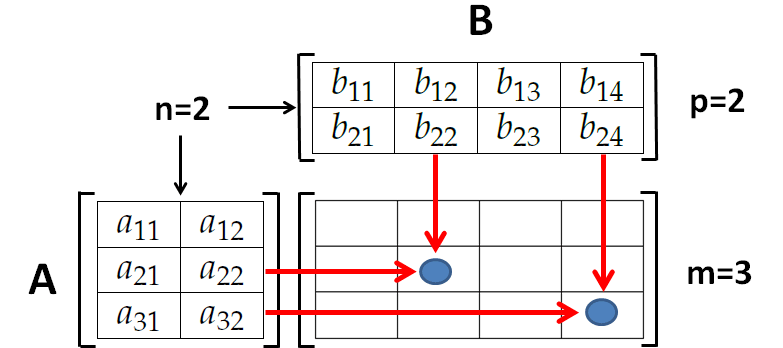
\includegraphics[height=6cm]{diagram/intro.png}
    

\caption{Matrix multiplication as a fundamental computational primitive in modern computing systems.\cite{fig_matrix_multiplication_bagdasar}}
\end{figure}

Despite its importance, matrix multiplication can be computationally expensive when executed on traditional scalar processors. 
General-purpose CPUs execute instructions sequentially, typically performing one arithmetic operation at a time. 
When implementing matrix multiplication in software, the computation is usually expressed as nested loops that repeatedly perform multiplication and addition operations. 
For embedded processors with limited computational resources, this sequential execution leads to a high number of clock cycles for even small matrix sizes.

Lightweight processors such as compact RISC-V cores are particularly affected by this limitation~\cite{asanovic2014instruction}.
While these processors provide flexibility and programmability, they are not optimized for performing large numbers of parallel arithmetic operations. 
As a result, executing matrix multiplication entirely in software can significantly increase execution time and reduce system efficiency.

To overcome these limitations, many modern computing architectures incorporate \textbf{hardware accelerators}. 
Hardware accelerators are specialized computation units designed to perform specific tasks more efficiently than a general-purpose processor. 
By implementing critical computational kernels directly in hardware, accelerators can exploit parallelism and reduce the number of clock cycles required for computation.

\section{Problem Statement}

The primary challenge addressed in this project is the \textbf{inefficiency of software-based matrix multiplication on compact RISC-V processors}. 
When matrix multiplication is executed purely in software, the processor must repeatedly fetch instructions, decode them, and execute individual arithmetic operations for each element of the matrix. 
This process results in a large number of instructions and consequently a high execution latency.

Several key limitations arise in this context:

\begin{itemize}
    \item \textbf{High cycle cost of scalar computation:} Each multiplication and addition operation must be executed sequentially by the processor.
    
    \item \textbf{Limited computational parallelism:} General-purpose processors typically perform one arithmetic operation per instruction cycle, which restricts the level of parallel computation.
    
    \item \textbf{Inefficient utilization of hardware resources:} Performing matrix operations through software loops does not fully exploit the potential parallelism available in hardware.
    
    \item \textbf{Need for seamless CPU integration:} Any hardware acceleration mechanism must integrate cleanly with the processor so that it can be invoked through software while maintaining normal instruction flow.
\end{itemize}

Therefore, the core problem addressed in this project is the design of a \textbf{hardware-based matrix multiplication accelerator} that can significantly reduce the number of clock cycles required for matrix computation while remaining tightly integrated with a RISC-V processor.

\section{Proposed Approach}

To address the computational limitations of software-based matrix multiplication, this project proposes the design of a \textbf{dedicated matrix multiplication accelerator integrated as a coprocessor with a RISC-V CPU}. 
Instead of executing matrix multiplication using nested software loops, the processor offloads the computation to a specialized hardware unit capable of performing multiple arithmetic operations in parallel.

The system architecture integrates a lightweight RISC-V processor core, \textbf{PicoRV32}, with a custom hardware accelerator. 
Communication between the CPU and the accelerator is implemented using the \textbf{Pico Co-Processor Interface (PCPI)}, which allows custom instructions to trigger external hardware modules. 
Through this interface, the processor can delegate matrix computation tasks to the accelerator while temporarily stalling execution until the result becomes available.

\begin{figure}[h]
\centering

    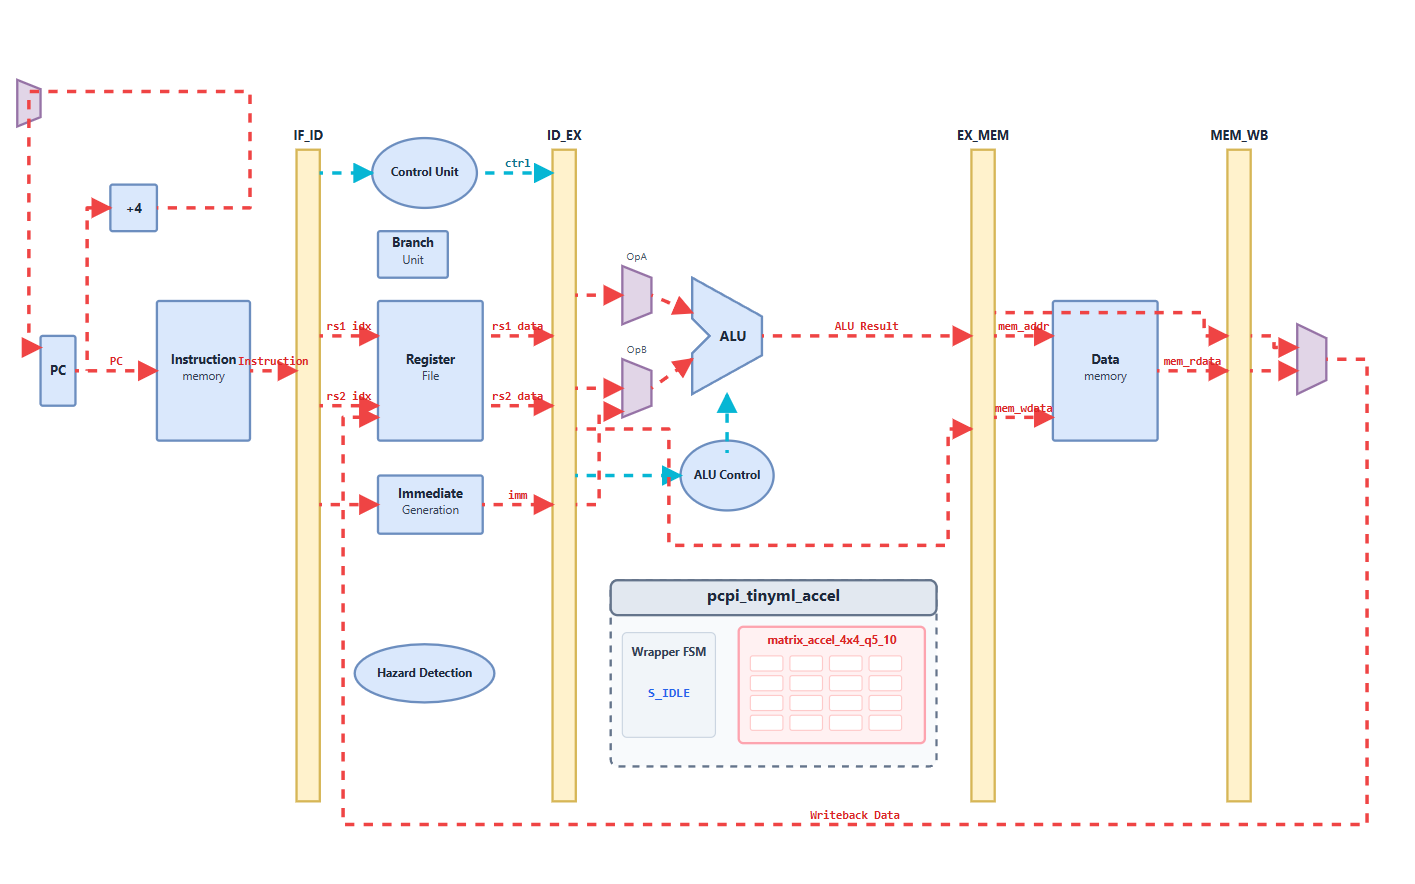
\includegraphics[height=9cm]{diagram/tinyml_accelerator_detailed_architecture.png}
    

\caption{High-level architecture of the RISC-V system with a matrix multiplication coprocessor.\cite{kaif2026visualizer_overview}}
\end{figure}

The matrix accelerator itself is implemented using a \textbf{systolic array architecture}. 
A systolic array consists of a grid of processing elements that perform multiply–accumulate operations while passing intermediate data between neighboring cells in a synchronized pipeline~\cite{kung1979systolic}.
This architecture enables high levels of parallelism and efficient data reuse, making it particularly well suited for matrix computations.

Each processing element performs arithmetic operations using a \textbf{Q5.10 fixed-point representation}. 
Fixed-point arithmetic is chosen instead of floating-point arithmetic in order to reduce hardware complexity and improve computational efficiency for embedded systems.

\section{Project Scope and Current Stage}

The objective of this project is to design and implement a \textbf{compact hardware accelerator for matrix multiplication integrated with a RISC-V processor}. 
The accelerator is designed to support a $4 \times 4$ matrix multiplication operation and can be invoked through a custom instruction executed by the CPU.

The project follows a \textbf{simulation-driven development methodology}. 
All hardware components are implemented using Verilog and verified through a comprehensive simulation environment. 
The simulation framework includes a processor model, firmware execution, and automated verification of computational results.

The current implementation includes:

\begin{itemize}
    \item Design of the hardware matrix multiplication accelerator using a systolic array architecture.
    \item Integration of the accelerator with the PicoRV32 RISC-V core through the PCPI interface.
    \item Development of firmware that initializes input matrices and invokes the accelerator using a custom instruction.
    \item Creation of a structured simulation testbench for functional verification.
    \item Performance comparison between software-based matrix multiplication and hardware-accelerated execution.
\end{itemize}

Future work will focus on extending the design toward \textbf{FPGA deployment}, enabling execution on physical hardware platforms and allowing measurement of real-world performance metrics such as latency, throughput, and power efficiency.

Overall, this project demonstrates how integrating a specialized matrix computation accelerator as a coprocessor within a RISC-V system can significantly improve the efficiency of numerical workloads while maintaining programmability and architectural simplicity.

% ============================================================
%  Chapter: Related Work
%  Insert this chapter AFTER \chapter{Introduction} and
%  BEFORE \chapter{System Architecture and Implementation}.
%
%  In your main .tex preamble, add (if not already present):
%    \usepackage{cite}          % or natbib / biblatex
%    \usepackage{graphicx}      % already in your preamble
%    \usepackage{booktabs}      % already in your preamble
%    \usepackage{tabularx}      % already in your preamble
%    \usepackage{float}         % already in your preamble
%
%  At the end of your main .tex document (before \end{document}),
%  replace or supplement any existing bibliography commands with:
%    \bibliographystyle{IEEEtran}
%    \bibliography{tacr_references}
% ============================================================

% ============================================================
%  Chapter: Related Work
%  Insert this chapter AFTER \chapter{Introduction} and
%  BEFORE \chapter{System Architecture and Implementation}.
%
%  In your main .tex preamble, add (if not already present):
%    \usepackage{cite}          % or natbib / biblatex
%    \usepackage{graphicx}      % already in your preamble
%    \usepackage{booktabs}      % already in your preamble
%    \usepackage{tabularx}      % already in your preamble
%    \usepackage{float}         % already in your preamble
%
%  At the end of your main .tex document (before \end{document}),
%  replace or supplement any existing bibliography commands with:
%    \bibliographystyle{IEEEtran}
%    \bibliography{tacr_references}
% ============================================================

% ============================================================
%  Chapter: Related Work
%  Insert this chapter AFTER \chapter{Introduction} and
%  BEFORE \chapter{System Architecture and Implementation}.
%
%  In your main .tex preamble, add (if not already present):
%    \usepackage{cite}          % or natbib / biblatex
%    \usepackage{graphicx}      % already in your preamble
%    \usepackage{booktabs}      % already in your preamble
%    \usepackage{tabularx}      % already in your preamble
%    \usepackage{float}         % already in your preamble
%
%  At the end of your main .tex document (before \end{document}),
%  replace or supplement any existing bibliography commands with:
%    \bibliographystyle{IEEEtran}
%    \bibliography{tacr_references}
% ============================================================

\chapter{Related Work}

\section{Introduction}

The EdgeMATX project draws on four
active research areas:
(i)~systolic-array hardware design for matrix multiplication,
(ii)~RISC-V custom instruction extensions and CPU--accelerator
co-design,
(iii)~fixed-point arithmetic for hardware-efficient computation, and
(iv)~the broader landscape of application-specific accelerators
targeting workloads---such as machine learning---that are dominated
by matrix operations.
The project itself focuses entirely on hardware design and
simulation; no ML model training or inference testing is performed.
This chapter reviews representative and recent literature across all
four areas, situating each design decision and quantifying how EdgeMATX
compares to the state of the art.

% -----------------------------------------------------------
\section{Systolic Array Architectures for Matrix Multiplication}
% -----------------------------------------------------------

Matrix multiplication is the dominant arithmetic kernel in a wide
class of compute-intensive workloads, including signal processing,
scientific computing, and machine learning.
Hardware acceleration via systolic arrays has been studied for
decades, but recent years have seen a surge of FPGA-targeted,
parameterisable implementations driven by the growing demand for
efficient compute at the edge.
EdgeMATX adopts this approach, implementing a $4\times4$ systolic engine
in Verilog as the core compute tile.

\begin{figure}[H]
  \centering
  % ----------------------------------------------------------
  % INSERT IMAGE HERE
  % Suggested file: fig_systolic_array.png
  % Export from Draw.io / PowerPoint at >= 1800 px width.
  % ----------------------------------------------------------
  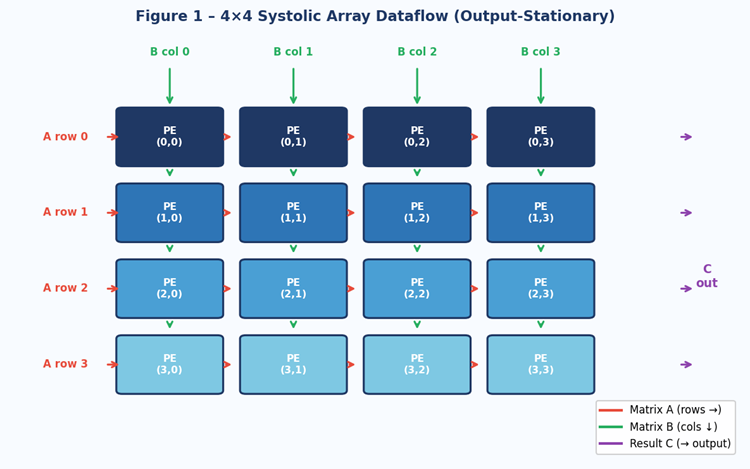
\includegraphics[width=0.82\textwidth]{figures/fig_systolic_array.png}
  \caption{Canonical $4\times4$ systolic array dataflow.
           Data from matrix $A$ streams across rows (red arrows)
           and data from matrix $B$ streams down columns
           (green arrows); each PE performs one MAC per cycle and
           forwards its inputs to its neighbours.
           This is the topology employed in the EdgeMATX engine.
           (Adapted from~\cite{mattimani2024fpga}.)}
  \label{fig:systolic_array}
\end{figure}

\subsection{FPGA Systolic Array Implementations}

Mattimani~\textit{et al.}~\cite{mattimani2024fpga} present a
parameterisable FPGA systolic array for matrix multiplication,
demonstrating that FPGA parallelism and pipelining together yield
substantial speed-up over sequential software.
They emphasise resource sharing and data-movement minimisation---
principles directly mirrored in the Q5.10 fixed-point design of
EdgeMATX.

Shapri~\textit{et al.}~\cite{shapri2024optimization} report an
optimised Verilog-based systolic array simulated in Quartus Prime,
with power-optimisation results showing reduced dissipation and
area.
Their use of 3-bit ALU benchmarking underscores the need for
rigorous characterisation of the processing-element arithmetic, a
practice replicated in EdgeMATX via regression-driven simulation in
Icarus Verilog.


Wei~\textit{et al.}~\cite{wei2024faulttolerant} tackle fault-tolerant
systolic execution via a pair-matching mechanism, demonstrating
that systolic reliability becomes significant as array size grows---a
concern relevant to any future scale-up of the EdgeMATX accelerator.
Their Cannon's-algorithm-based architecture also illustrates
alternative dataflow choices to the output-stationary scheme used
in EdgeMATX.

\subsection{Systolic Arrays in Application-Specific Contexts}

Ye~\textit{et al.}~\cite{ye2023highfrequency} propose a
high-frequency systolic-array accelerator on FPGA for
Transformer workloads, achieving $474$--$588\,$MHz and
$1.5$--$1.8\times$ frequency improvement over prior work on a
Xilinx ZCU102.
This confirms that systolic arrays are the canonical compute tile
for GEMM-heavy workloads on FPGAs---the central architectural
premise of EdgeMATX---and provides concrete timing benchmarks that
inform expected frequency targets for the planned Pynq-Z2
deployment.


% -----------------------------------------------------------
\section{RISC-V Custom Instructions and CPU--Accelerator Co-design}
% -----------------------------------------------------------

\begin{figure}[H]
  \centering
  % ----------------------------------------------------------
  % INSERT IMAGE HERE
  % Suggested file: fig_pcpi_handshake.png
  % ----------------------------------------------------------
  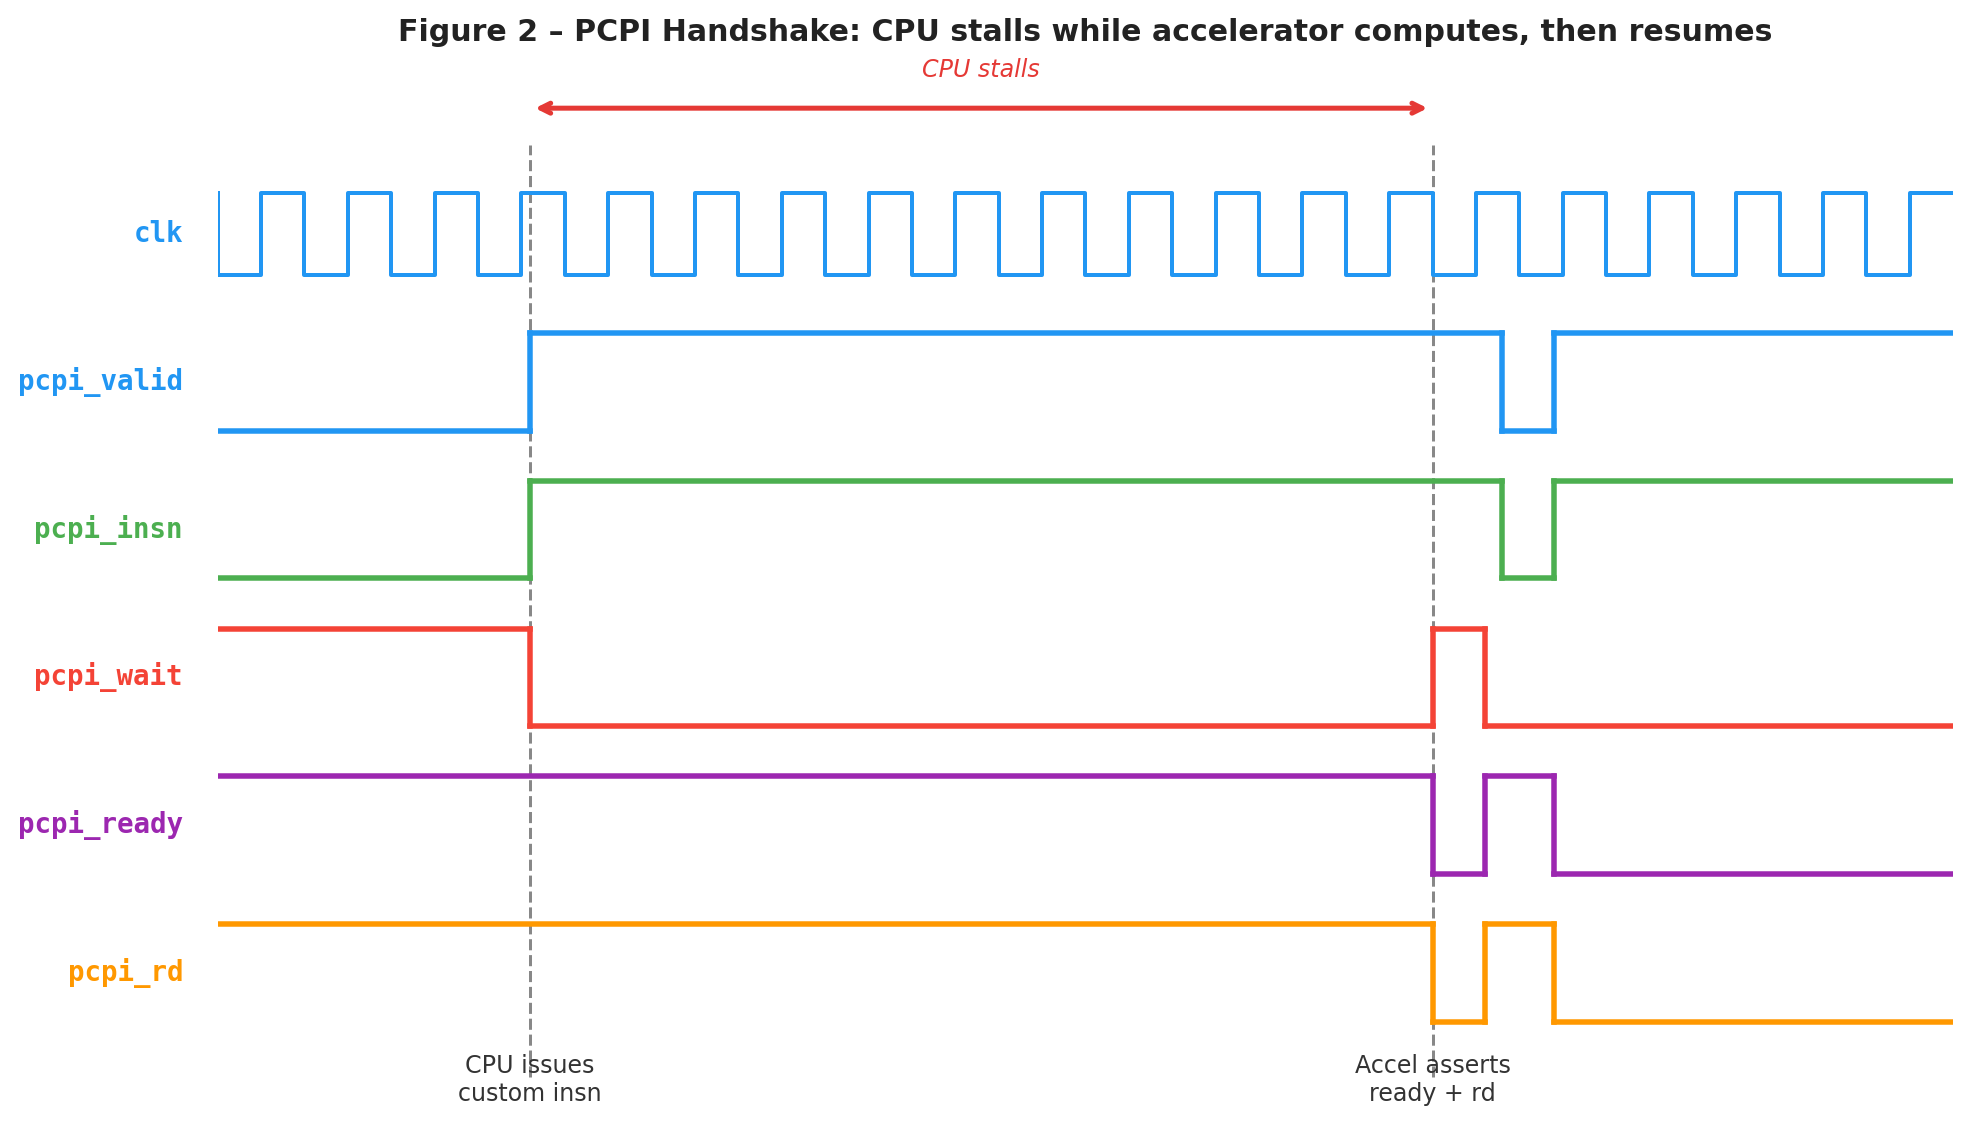
\includegraphics[width=0.82\textwidth]{figures/fig_pcpi_handshake.png}
  \caption{PCPI handshake timing diagram.
           The CPU stalls (\texttt{pcpi\_wait} high) from the cycle
           it issues the custom instruction until the accelerator
           asserts \texttt{pcpi\_ready} and places the result on
           \texttt{pcpi\_rd}.
           This is exactly the protocol implemented in EdgeMATX.
           (Adapted from~\cite{wolf2024picorv32}.)}
  \label{fig:pcpi_handshake}
\end{figure}

\subsection{The PicoRV32 PCPI Interface}

The PicoRV32~\cite{wolf2024picorv32} is a size-optimised,
open-source RV32I soft-core that exposes the Pico Co-Processor
Interface (PCPI)---a lightweight handshake
(\texttt{pcpi\_valid}, \texttt{pcpi\_insn},
\texttt{pcpi\_rs1}/\texttt{rs2},
\texttt{pcpi\_ready}, \texttt{pcpi\_wait}, \texttt{pcpi\_rd})
enabling external hardware to implement custom non-branching
instructions with minimal CPU modification.
The CPU stalls on any unrecognised instruction, asserting
\texttt{pcpi\_valid}; the co-processor must respond within
16 cycles (or hold \texttt{pcpi\_wait} to extend the stall
indefinitely).
This interface is the integration backbone of the EdgeMATX
PCPI demo.


\subsection{RISC-V ISA Extensions for Compute-Intensive Workloads}

Balasubramanian~\textit{et al.}~\cite{balasubramanian2024riscv}
survey the design of RISC-V ISA extensions for compute-intensive
workloads from a compiler perspective, presenting an LLVM-based
toolchain that automatically lowers computation graphs to custom
instructions.
They find that ISA extensions can reduce cycle count by
$30$--$50\%$ with minimal hardware overhead.
EdgeMATX does not implement a compiler toolchain, but the
$38$--$54\times$ cycle-count improvement it measures over
software baselines is consistent with and exceeds these figures,
confirming that the custom-instruction approach is architecturally
well-founded.

Salinas~\textit{et al.}~\cite{salinas2024custom} investigate
custom ISA extensions for data-intensive load/store operations
on RISC-V, achieving approximately $50\%$ cycle reduction and
$30\%$ power reduction.
Their approach targets the memory-bandwidth bottleneck that often
limits achievable speed-up once compute is accelerated---a
bottleneck that will become relevant as EdgeMATX scales beyond
$4\times4$ matrices to larger problem sizes.

Sharma~\textit{et al.}~\cite{sharma2022extremedge} provide a
systematic hardware/software co-design methodology
(EXTREM-EDGE) for integrating arithmetic functional units as
tightly coupled extensions to RISC-V, yielding
$1.75\times$--$17.63\times$ kernel-level improvements and
$1.41\times$--$4.41\times$ full-application cycle reductions.
This co-design philosophy---where a custom instruction directly
triggers an accelerator operation---is the architectural pattern
adopted in the EdgeMATX PCPI demo, and this work validates it as a
sound design strategy.


Finally, \cite{anon2025fpgariesv} presents a complete
FPGA-accelerated RISC-V system on the Pynq-Z2 board---the same
target platform planned for EdgeMATX---with verified AXI
interconnect, BRAM memory access, and timing closure at
$50\,$MHz, providing direct evidence that a RISC-V +
custom-accelerator system can be fully integrated and measured on
Pynq-Z2 hardware.

% -----------------------------------------------------------
\section{Fixed-Point Arithmetic and Numerical Representation}
% -----------------------------------------------------------

\begin{figure}[H]
  \centering
  % ----------------------------------------------------------
  % INSERT IMAGE HERE
  % Suggested file: fig_qformat.png
  % ----------------------------------------------------------
  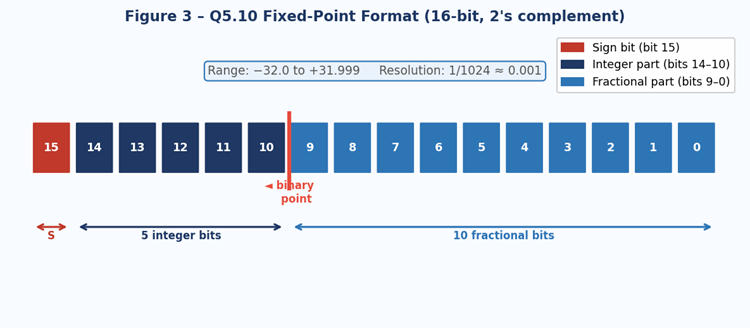
\includegraphics[width=0.78\textwidth]{figures/fig_qformat.png}
  \caption{Q5.10 fixed-point format (16-bit, two's complement).
           Bit~15 is the sign bit; bits~14--10 carry the integer
           part; bits~9--0 carry the fractional part.
           Range: $-32.0$ to $+31.999$; resolution:
           $1/1024 \approx 0.001$.
           (Adapted from~\cite{nguyen2023qformat}.)}
  \label{fig:qformat}
\end{figure}

Hardware accelerators must operate on compact numerical
representations to fit within the resource budgets of edge FPGAs.
The Q-format fixed-point scheme---where a fixed binary-point
position divides a two's-complement integer word into integer and
fractional fields---is the standard approach for FPGA-based
arithmetic accelerators because it maps multiplications directly
to DSP slices with no floating-point overhead.
EdgeMATX uses Q5.10, a 16-bit format that balances dynamic range and
fractional precision for the matrix operand values targeted in
simulation.

\subsection{Q-Format Arithmetic}

Nguyen~\textit{et al.}~\cite{nguyen2023qformat} study hybrid
Q-format fixed-point multiplication for FPGA accelerators,
integrating sign-bit check and bit round-off into the multiply
path to address overflow.
They identify Q(6.9) as near-optimal for their target operand
range, showing that fractional bit-width must be chosen in
proportion to the expected input dynamic range.
EdgeMATX's Q5.10 selection follows the same reasoning: sufficient
fractional precision to preserve numerical accuracy across typical
matrix operand magnitudes, while keeping the datapath to 16 bits.

Dai~\textit{et al.}~\cite{dai2024qfx} present QFX, a trainable
fixed-point quantisation library for FPGAs that automates
binary-point selection.
While EdgeMATX's Q5.10 format is manually chosen for simulation, this
work points to a future toolflow path for systematically
determining the optimal format when deploying real workloads on
the Pynq-Z2 hardware.

\subsection{Fixed-Point Design for FPGAs}

Zhang~\textit{et al.}~\cite{matinizadeh2025quantized}
publish a comprehensive hardware-perspective survey of
fixed-point accelerators on ASIC and FPGA platforms.
The survey confirms that systolic-array-based implementations with
16-bit or sub-16-bit fixed-point arithmetic achieve the best
energy-area trade-off on FPGAs, consistent with the 16-bit Q5.10
design choice in EdgeMATX.
It also documents the resource savings available by moving from
floating-point to fixed-point arithmetic, quantifying DSP and LUT
reductions that directly apply to the Pynq-Z2 deployment target.

Tasci~\textit{et al.}~\cite{alshedivat2025fpgaqnn} present
FPGA-QNN, demonstrating that multi-bit fixed-point compute engines
achieve substantial reductions in DSP and BRAM usage without
sacrificing arithmetic correctness.
Their results reinforce the viability of sub-16-bit computation on
resource-constrained FPGAs, and suggest that a future 8-bit variant
of the EdgeMATX engine would be both feasible and more area-efficient.

% -----------------------------------------------------------
\section{Application Context: Matrix Acceleration for Compute-Intensive Workloads}
% -----------------------------------------------------------

\begin{figure}[H]
  \centering
  % ----------------------------------------------------------
  % INSERT IMAGE HERE
  % Suggested file: fig_system_stack.png
  % ----------------------------------------------------------
  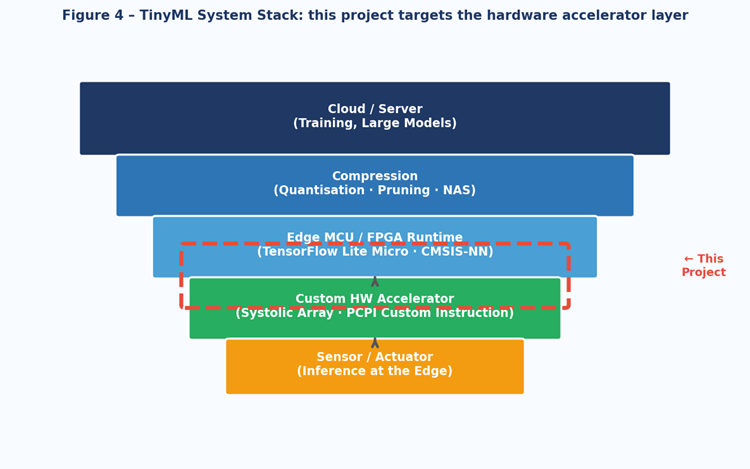
\includegraphics[width=0.72\textwidth]{figures/fig_system_stack.png}
  \caption{System stack for compute-intensive edge workloads.
           EdgeMATX targets the hardware accelerator layer
           (highlighted); no ML model deployment or inference
           testing is performed within the project scope.
           (Adapted from~\cite{osman2022tinyml}.)}
  \label{fig:system_stack}
\end{figure}

Although EdgeMATX performs no ML testing, the application domain that
drives demand for hardware GEMM acceleration provides important
context for the architectural choices made.

\subsection{Motivation: Why Matrix Acceleration Matters}

Osman~\textit{et al.}~\cite{osman2022tinyml} survey hardware
acceleration requirements for inference on constrained devices,
reporting that the dominant execution time is consumed by
matrix-multiply and convolution kernels---precisely the operation
EdgeMATX accelerates.
Their analysis establishes the memory and throughput budgets within
which a hardware GEMM engine must operate to be practically useful.

Somvanshi~\cite{saha2025tinydl} survey hardware
platforms for compute-intensive deep learning, presenting a
taxonomy that places dedicated arithmetic accelerators---such as
systolic arrays---as achieving up to $20\times$ performance
improvement over general-purpose processor implementations.
EdgeMATX's measured $38\times$ cycle-count reduction over a plain
RV32I software baseline comfortably exceeds this figure,
validating the design from a purely hardware-performance
standpoint, independent of any end-to-end application benchmark.


\subsection{Related Hardware Accelerator Designs}

Adithya Krishna~\textit{et al.}~\cite{saiteja2024raman} present RAMAN,
a reconfigurable sparse FPGA accelerator that exploits both weight
and activation sparsity, outperforming prior art in latency and
energy efficiency.
Its architectural analysis---which identifies memory-hierarchy
management as the critical bottleneck after the compute array is
optimised---directly informs the next development phase of EdgeMATX,
where AXI-based BRAM access on the Pynq-Z2 will become the
primary performance constraint.

Bhushan~\textit{et al.}~\cite{moosmann2025deploying} profile
fixed-point arithmetic accelerators on low-power edge FPGAs,
demonstrating that integer compute engines achieve substantial
latency and energy reductions over floating-point baselines.
Their profiling methodology---measuring cycles on hardware with
on-chip counters---is the same approach planned for the EdgeMATX
Pynq-Z2 deployment phase, where the simulation-based cycle counts
will be validated against real board measurements.

Pazmi\~{n}o~\textit{et al.}~\cite{manzoni2025advancing} survey
system-level challenges in deploying compute acceleration on edge
devices, explicitly discussing the trade-off between loosely
coupled (AXI/DMA) and tightly coupled (custom instruction)
accelerator interfaces---the exact design choice made in EdgeMATX.
They conclude that tightly coupled interfaces offer lower latency
for small, frequently-invoked kernels, as in the $4\times4$
matrix multiply case.


\chapter{System Architecture and Implementation}

\section{Overall System Architecture}

The proposed system integrates a lightweight RISC-V processor with a dedicated hardware accelerator for matrix multiplication. 
The accelerator is implemented as a coprocessor connected to the CPU through the \textbf{Pico Co-Processor Interface (PCPI)}. 
This interface allows the processor to invoke the accelerator using a custom instruction while maintaining normal instruction flow.

The overall architecture consists of the following major components:

\begin{itemize}
    \item \textbf{RISC-V CPU Core}: PicoRV32 processor responsible for program execution.
    \item \textbf{PCPI Coprocessor Wrapper}: Interface logic that connects the CPU to the accelerator.
    \item \textbf{Matrix Accelerator}: Dedicated hardware module implementing matrix multiplication.
    \item \textbf{Systolic Array Datapath}: Parallel computation engine composed of processing elements.
    \item \textbf{Firmware Layer}: Software running on the CPU that initializes data and triggers accelerator execution.
\end{itemize}

\begin{figure}[H]
\centering
 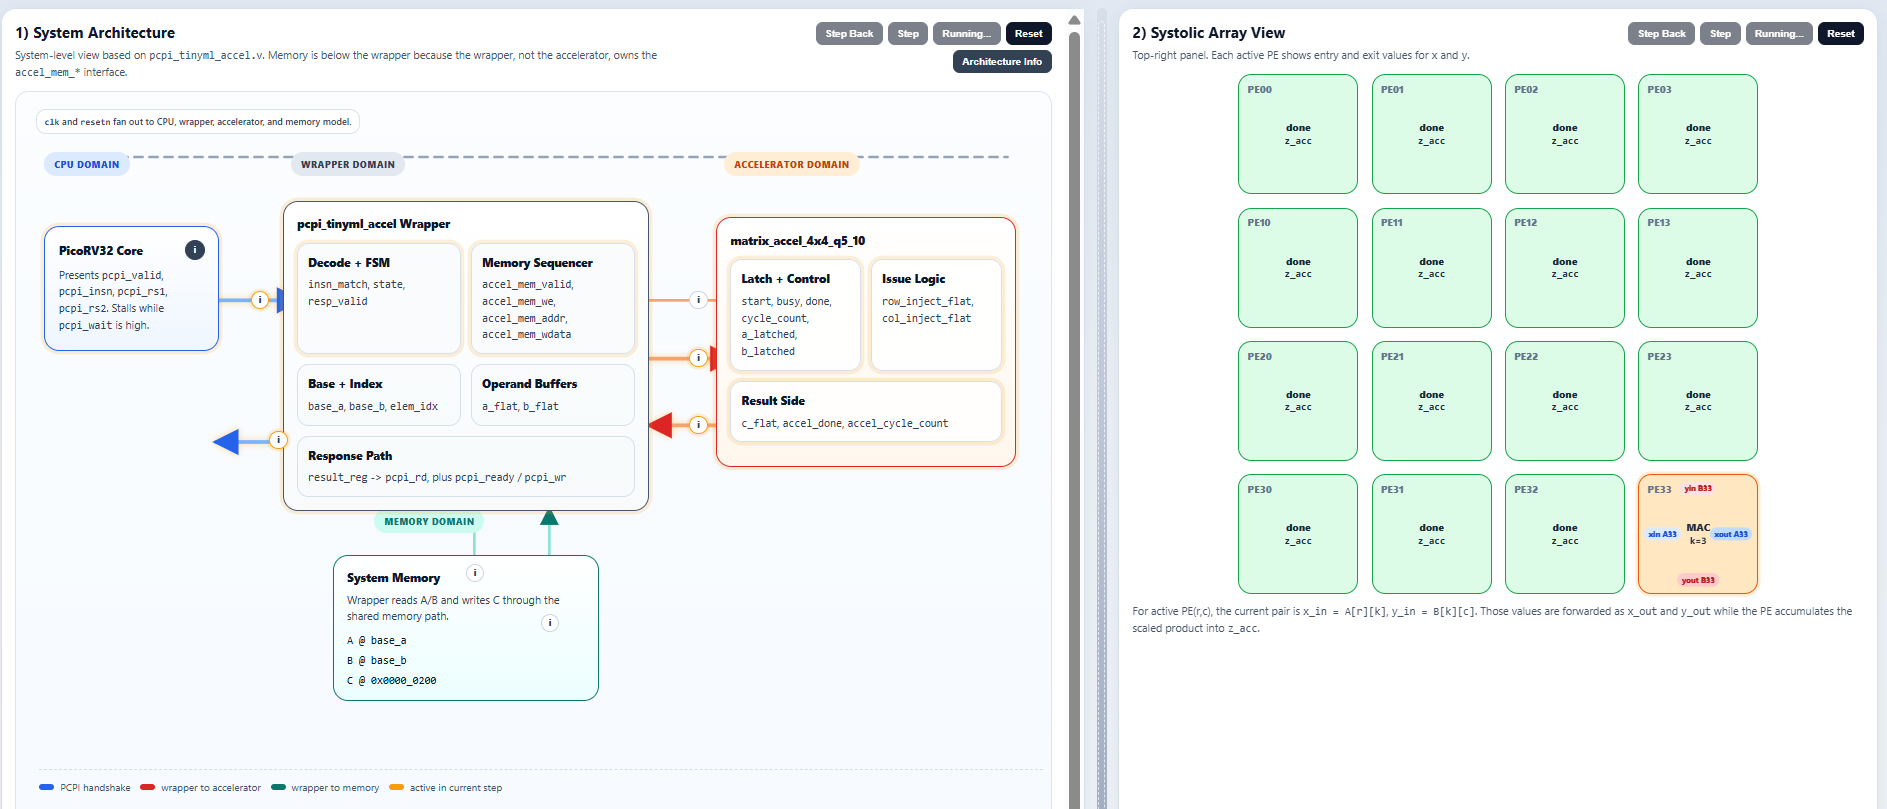
\includegraphics[height=7cm]{diagram/block_diag.png}
\caption{High-level system architecture of the RISC-V processor with the matrix multiplication coprocessor.\cite{kaif2026visualizer_signals}}
\end{figure}

For interactive exploration of the architecture and execution flow, two web-based visualization tools are provided. 
The first visualization presents the \textbf{high-level system architecture and dataflow}, while the second visualization shows the \textbf{detailed processor-level operation including internal signals, PCPI interaction, and systolic accelerator behavior}.

\begin{figure}[H]
\centering
\fbox{
\begin{minipage}{0.9\textwidth}
\centering
\textbf{Interactive System Visualizations}

\vspace{0.5cm}

\textbf{Architecture Overview Visualization}

\vspace{0.2cm}

This visualization illustrates the high-level system architecture including the firmware layer, PicoRV32 processor, PCPI coprocessor interface, and matrix accelerator datapath.

\vspace{0.2cm}

\href{https://riscv-visualizer-2.vercel.app/}{\texttt{Open Architecture Overview}}

\vspace{0.6cm}

\textbf{Processor and Signal-Level Visualization}

\vspace{0.2cm}

This visualization demonstrates the internal execution behavior of the processor including instruction decoding, PCPI signaling, accelerator invocation, and systolic array computation signals.

\vspace{0.2cm}

\href{https://tinyml-pcpi-visualizer.vercel.app}{\texttt{Open Detailed Processor Simulation}}

\end{minipage}
}
\caption{Interactive web-based visualizations for system architecture and detailed processor–accelerator execution flow.}
\label{fig:interactive_visualizations}
\end{figure}

\section{Matrix Accelerator Architecture}

The hardware accelerator is designed to compute a $4 \times 4$ matrix multiplication using a dedicated datapath implemented in Verilog. 
Instead of executing matrix multiplication through nested software loops, the CPU offloads the computation to the accelerator using a custom instruction.

The accelerator contains three primary internal modules:

\begin{itemize}
    \item \textbf{Issue Logic}: Responsible for scheduling and injecting matrix elements into the systolic array.
    \item \textbf{Systolic Array}: Parallel processing grid performing multiply–accumulate operations.
    \item \textbf{Processing Elements (PEs)}: Individual computation units that perform arithmetic operations.
\end{itemize}

\begin{figure}[H]
\centering
 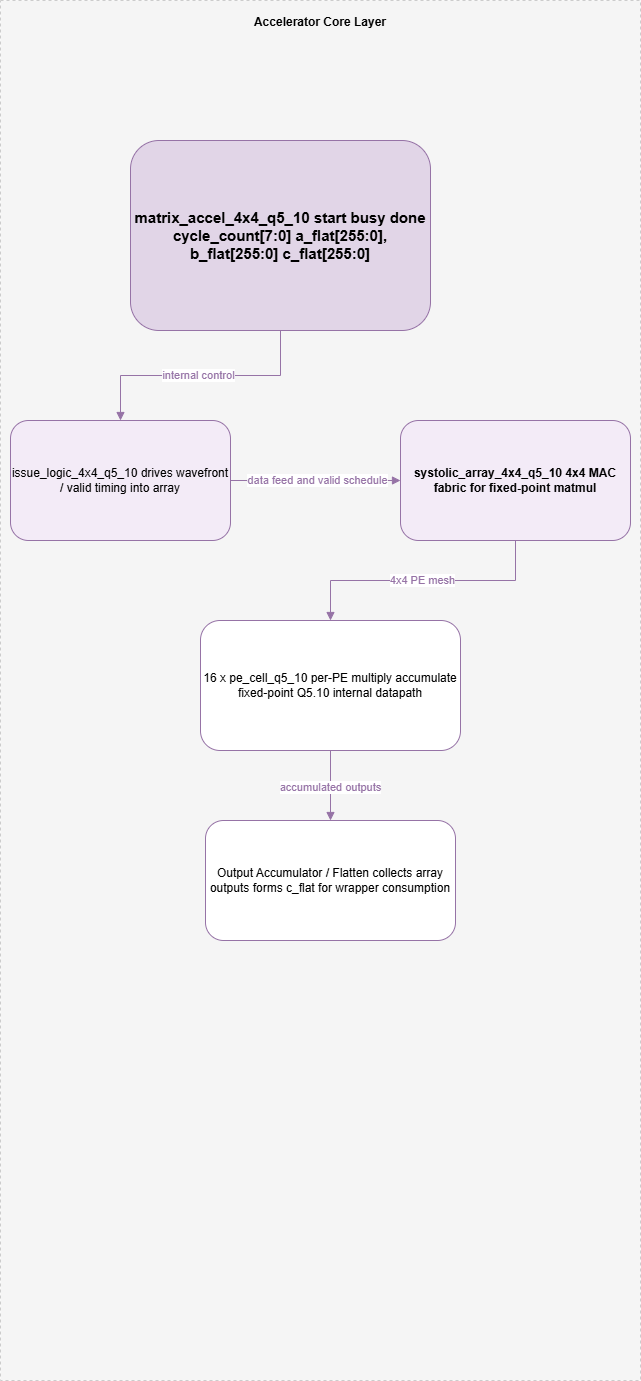
\includegraphics[height=9cm]{diagram/accelerator_arch.png}
\caption{Internal architecture of the matrix multiplication accelerator.}
\end{figure}

The accelerator follows a \textbf{systolic computation model}, where data flows rhythmically through a grid of processing elements. 
Each processing element performs multiplication and accumulation operations while forwarding partial results to neighboring cells.

\section{Systolic Array Architecture}

The computation engine of the accelerator is implemented using a $4 \times 4$ systolic array composed of 16 processing elements. 
In a systolic array, data propagates through the array in a pipelined fashion, enabling multiple arithmetic operations to be executed simultaneously.

Matrix elements from input matrices $A$ and $B$ are injected into the array from orthogonal directions. 
As the data flows across the array, each processing element computes partial products and accumulates them to produce the final output matrix.

The mathematical operation performed is given by:

\begin{equation}
C_{i,j} = \sum_{k=1}^{4} A_{i,k} \times B_{k,j}
\end{equation}

\begin{figure}[H]
\centering
 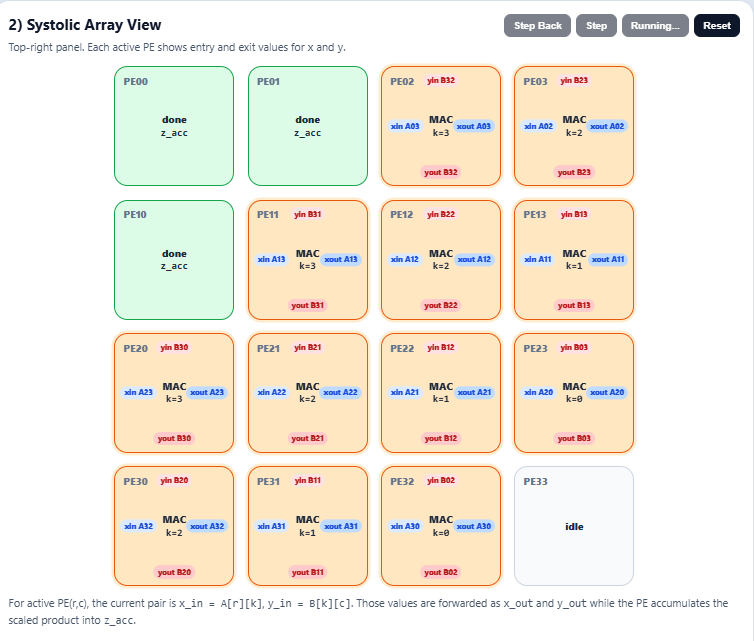
\includegraphics[height=9cm]{diagram/systolic.png}
\caption{Internal architecture of the matrix multiplication accelerator.\cite{kaif2026visualizer_signals}}
\end{figure}

\section{Processing Element Design}

Each processing element (PE) performs the core multiply–accumulate operation. 
The PE receives input values from neighboring cells, computes a scaled multiplication using fixed-point arithmetic, and accumulates the result.

The arithmetic follows a \textbf{Q5.10 fixed-point format}, where numbers are represented using a signed 16-bit representation with 10 fractional bits.

The PE performs the following steps:

\begin{enumerate}
    \item Multiply two signed 16-bit inputs.
    \item Perform arithmetic right shift by 10 bits to maintain fixed-point scaling.
    \item Accumulate the result into a 32-bit register.
    \item Forward the input values to neighboring processing elements.
\end{enumerate}

\subsection{Processing Element Code Snippet}

\begin{lstlisting}[language=Verilog]
module pe_cell_q5_10(
    input clk,
    input rst,
    input signed [15:0] x_in,
    input signed [15:0] y_in,
    output signed [15:0] x_out,
    output signed [15:0] y_out
);

wire signed [31:0] mult;
assign mult = (x_in * y_in) >>> 10;

always @(posedge clk) begin
    acc <= acc + mult;
end

endmodule
\end{lstlisting}

\section{Issue Logic}

The issue logic module is responsible for scheduling matrix elements and feeding them into the systolic array at the correct clock cycles. 
It ensures that data elements from matrices $A$ and $B$ are injected into the array in a pattern that allows correct accumulation across the processing elements.

The module maintains a cycle counter and uses it to determine which matrix elements should be injected during each clock cycle.

\begin{lstlisting}[language=Verilog]
always @(posedge clk) begin
    if(start)
        cycle <= 0;
    else
        cycle <= cycle + 1;
end
\end{lstlisting}

This scheduling mechanism enables a pipelined computation where multiple matrix elements are processed concurrently.

\section{CPU–Accelerator Integration}

The accelerator is integrated with the PicoRV32 CPU using the \textbf{Pico Co-Processor Interface (PCPI)}. 
This interface allows custom instructions to trigger external hardware modules.

When the CPU encounters the custom instruction

\begin{verbatim}
.word 0x5420818b
\end{verbatim}

the PCPI wrapper intercepts the instruction and initiates accelerator execution.

The wrapper performs the following operations:

\begin{enumerate}
    \item Capture matrix base addresses from registers \texttt{rs1} and \texttt{rs2}.
    \item Read input matrix elements from memory.
    \item Trigger the accelerator computation.
    \item Wait for completion signal.
    \item Write the resulting matrix elements back to memory.
\end{enumerate}

\section{Execution Workflow}

The complete execution flow of the system is summarized below:

\begin{enumerate}
    \item Firmware loads matrix $A$ and matrix $B$ into memory.
    \item CPU executes the custom instruction that invokes the accelerator.
    \item PCPI wrapper decodes the instruction and captures matrix base addresses.
    \item Matrix elements are loaded into the accelerator datapath.
    \item The systolic array performs multiply–accumulate operations.
    \item The resulting matrix $C$ is written back to memory.
    \item CPU resumes execution of the remaining firmware instructions.
\end{enumerate}

\begin{figure}[H]
\centering
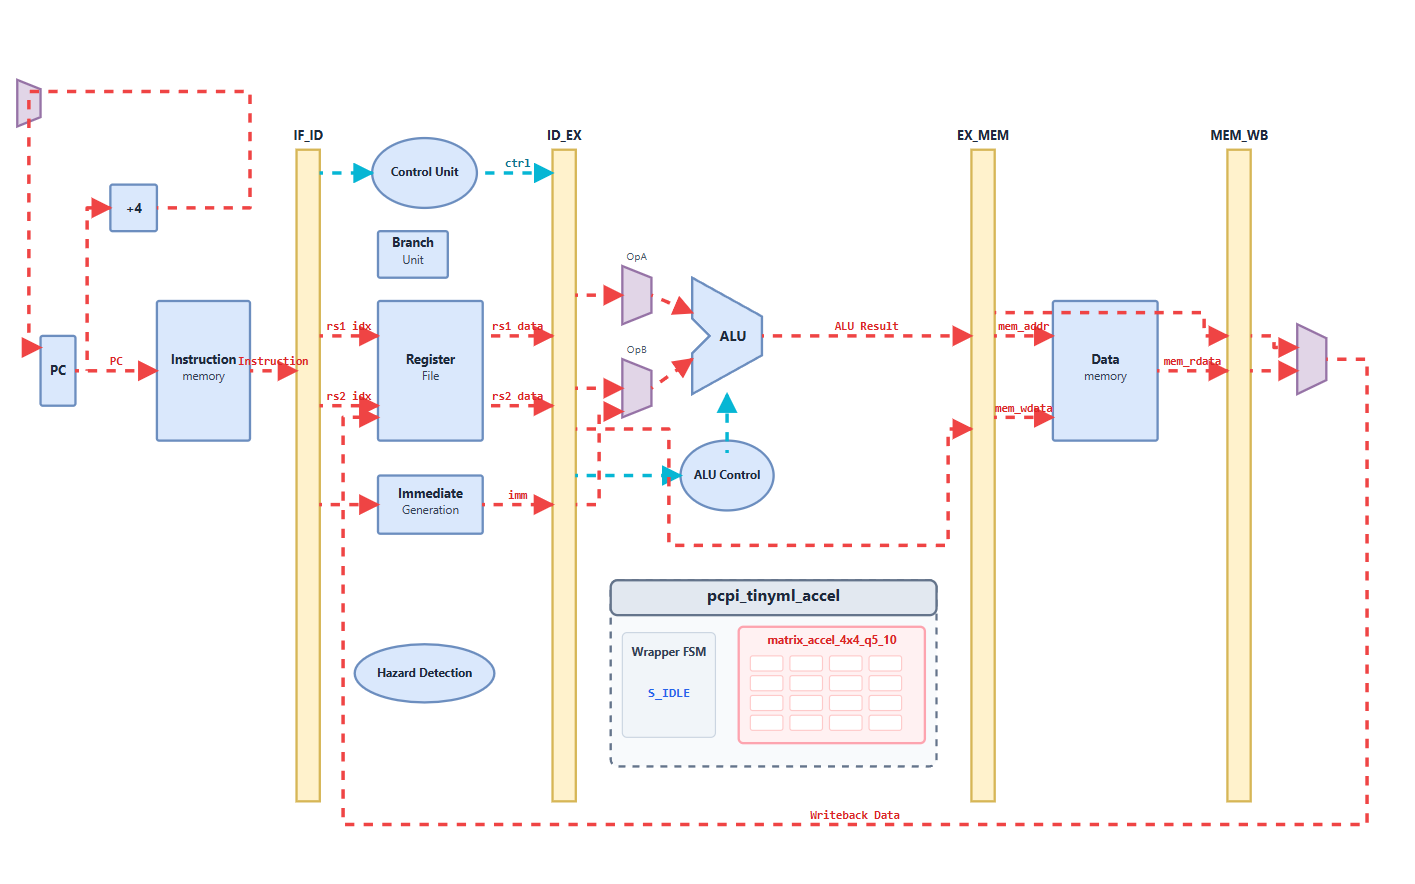
\includegraphics[height=9cm]{diagram/tinyml_accelerator_detailed_architecture.png}
\caption{Execution flow from custom instruction invocation to result writeback.\cite{kaif2026visualizer_overview}}
\end{figure}

\section{Memory Mapping}

The accelerator interacts with system memory through predefined memory regions used for storing input and output matrices.

\begin{table}[H]
\centering
\small
\begin{tabular}{lll}
\toprule
Region & Address Range & Purpose \\
\midrule
Matrix A & 0x100 -- 0x13C & Input elements of matrix A \\
Matrix B & 0x140 -- 0x17C & Input elements of matrix B \\
Matrix C & 0x200 -- 0x23C & Output elements of matrix C \\
Sentinel & 0x00000000 & Completion marker for testbench \\
\bottomrule
\end{tabular}
\caption{Memory layout used for matrix data exchange between CPU and accelerator.}
\end{table}

\section{Fixed-Point Arithmetic Contract}

All arithmetic operations follow a consistent fixed-point computation model:

\begin{enumerate}
    \item Signed 16-bit multiplication
    \item Arithmetic right shift by 10 bits for Q5.10 scaling
    \item Signed 32-bit accumulation
    \item Final truncation to lower 16 bits with sign extension for memory storage
\end{enumerate}

This arithmetic contract is preserved across both standalone accelerator simulations and integrated CPU execution flows to ensure consistent verification results.
% ================================================================
%  Chapter: Verification Methodology and Results
% ================================================================
\chapter{Verification Methodology and Results}

\section{Overview of Verification Approach}

The EdgeMATX verification strategy follows a structured, layered methodology that progressively validates the design from isolated hardware units to full system integration~\cite{bergeron2003writing}.
Rather than relying on a single monolithic simulation, the verification is decomposed into four distinct layers, each targeting a specific aspect of correctness:

\begin{enumerate}
    \item \textbf{Unit-level hardening:} Standalone accelerator functional correctness verified independently of the CPU and PCPI interface.
    \item \textbf{System-level integration:} CPU, PCPI wrapper, and matrix accelerator verified as a complete system under firmware-driven execution.
    \item \textbf{Protocol-level assurance:} PCPI handshake correctness validated with a mixed instruction stream, testing CPU stall and resume behavior across multiple consecutive custom instruction transactions.
    \item \textbf{Performance-level benchmarking:} Measured simulation cycle counts compared across the hardware-accelerated path and two software baselines to quantify speedup.
\end{enumerate}

This layered approach ensures that any failure is localized and attributable to a specific integration boundary, reducing debug overhead and improving coverage confidence.

\begin{figure}[H]
\centering
\fbox{%
\begin{minipage}[c][6.5cm][c]{0.88\textwidth}
\centering
\textbf{EdgeMATX Four-Layer Verification Hierarchy}\\[10pt]
\textbf{Layer 1} --- Standalone Accelerator (unit-level)\\[4pt]
$\downarrow$\\[4pt]
\textbf{Layer 2} --- CPU + PCPI Wrapper + Accelerator (system-level)\\[4pt]
$\downarrow$\\[4pt]
\textbf{Layer 3} --- Protocol Handoff: Mixed Instruction Stream (protocol-level)\\[4pt]
$\downarrow$\\[4pt]
\textbf{Layer 4} --- Cycle Comparison: Accelerator vs.\ Software Baselines (performance-level)\\[10pt]
\textit{Replace this box with a flowchart exported from Draw.io or PowerPoint.}
\end{minipage}}
\caption{Four-layer verification hierarchy for EdgeMATX.}
\label{fig:verif_hierarchy}
\end{figure}

% ----------------------------------------------------------------
\section{Verification Infrastructure and Tools}
% ----------------------------------------------------------------

All simulations are executed using \textbf{Icarus Verilog} (iverilog), an open-source Verilog simulator~\cite{williams_icarus_verilog}.
Firmware is compiled using the \textbf{RISC-V GNU toolchain}, targeting the \texttt{rv32i} ISA for software no-MUL baselines and custom-instruction paths, and \texttt{rv32im} when the hardware multiply extension is enabled.
Simulation logs are post-processed by automation scripts for pass/fail determination and cycle extraction.

The full verification infrastructure consists of the following reusable PowerShell scripts:

\begin{table}[H]
\centering
\small
\setlength{\tabcolsep}{6pt}
\renewcommand{\arraystretch}{1.3}
\begin{tabularx}{\textwidth}{
  >{\ttfamily\raggedright\arraybackslash}p{0.44\textwidth}
  >{\raggedright\arraybackslash}X
}
\toprule
\textbf{Script} & \textbf{Purpose} \\
\midrule
run\_midsem\_sim.ps1            & Standalone accelerator regression (19 test cases) \\
run\_pcpi\_demo.ps1             & Smoke test: ASM and C firmware variants \\
run\_pcpi\_regression.ps1       & 8-case integration regression suite \\
run\_pcpi\_handoff.ps1          & Protocol handoff with mixed instruction stream \\
run\_pcpi\_professor\_demo.ps1  & 5-case curated demonstration set \\
run\_pcpi\_local\_check.ps1     & One-command gate for quick correctness validation \\
run\_cycle\_compare.ps1         & Cycle measurement across all three execution paths \\
run\_pcpi\_custom\_cycle\_compare.ps1 & Live-input custom cycle comparison \\
\bottomrule
\end{tabularx}
\caption{Verification automation scripts and their roles.}
\label{tab:scripts}
\end{table}

% ----------------------------------------------------------------
\section{Layer 1 --- Standalone Accelerator Verification}
% ----------------------------------------------------------------

The first layer targets the matrix multiplication accelerator module in complete isolation, without the PicoRV32 CPU or PCPI wrapper.
Direct Verilog stimulus is applied to the accelerator inputs, and output values from the systolic array are compared against precomputed golden reference values.

\subsection{Test Configuration}

\begin{itemize}
    \item \textbf{Simulator:} Icarus Verilog
    \item \textbf{Script:} \texttt{run\_midsem\_sim.ps1}
    \item \textbf{Total test cases:} 19
    \item \textbf{Coverage:} Zero matrices, identity matrices, dense random matrices, Q5.10 edge values, sign-boundary operands, mixed-sign elements
\end{itemize}

\subsection{What Is Exercised}

\begin{itemize}
    \item Correctness of Q5.10 fixed-point multiply–accumulate (shift-by-10) in each processing element.
    \item Full 16-PE systolic array producing all 16 output elements of the $4 \times 4$ result.
    \item Correct operation of issue logic scheduling and its cycle-aligned data injection.
    \item Accumulator reset and output capture at the correct pipeline drain stage.
\end{itemize}

\subsection{Test Results by Category}

\begin{table}[H]
\centering
\small
\setlength{\tabcolsep}{8pt}
\renewcommand{\arraystretch}{1.3}
\begin{tabular}{lccl}
\toprule
\textbf{Category} & \textbf{Cases} & \textbf{Result} & \textbf{Date} \\
\midrule
Zero / null matrix             & 2  & PASS & 2026-03-05 \\
Identity matrix                & 3  & PASS & 2026-03-05 \\
Dense matrix (varied magnitudes) & 8 & PASS & 2026-03-05 \\
Q5.10 sign-boundary / edge     & 4  & PASS & 2026-03-05 \\
Negative-element operands      & 2  & PASS & 2026-03-05 \\
\midrule
\textbf{Total}                 & \textbf{19} & \textbf{PASS (19/19)} & \\
\bottomrule
\end{tabular}
\caption{Standalone accelerator test results by category.}
\label{tab:standalone_tests}
\end{table}

All 19 test cases passed, establishing unit-level confidence in the arithmetic correctness and timing of the accelerator datapath prior to CPU integration.

\subsection{Simulation Waveform}

Figure~\ref{fig:accel_waveform} shows the GTKWave capture from the standalone accelerator regression simulation~\cite{bybell_gtkwave}.
The view covers the first directed test case (\texttt{identity}): the reset deassertion, the \texttt{start} pulse, the fully-occupied computation window, the \texttt{done} assertion at cycle~10, and the appearance of the packed output on \texttt{c\_flat[255:0]}.

\begin{figure}[H]
\centering
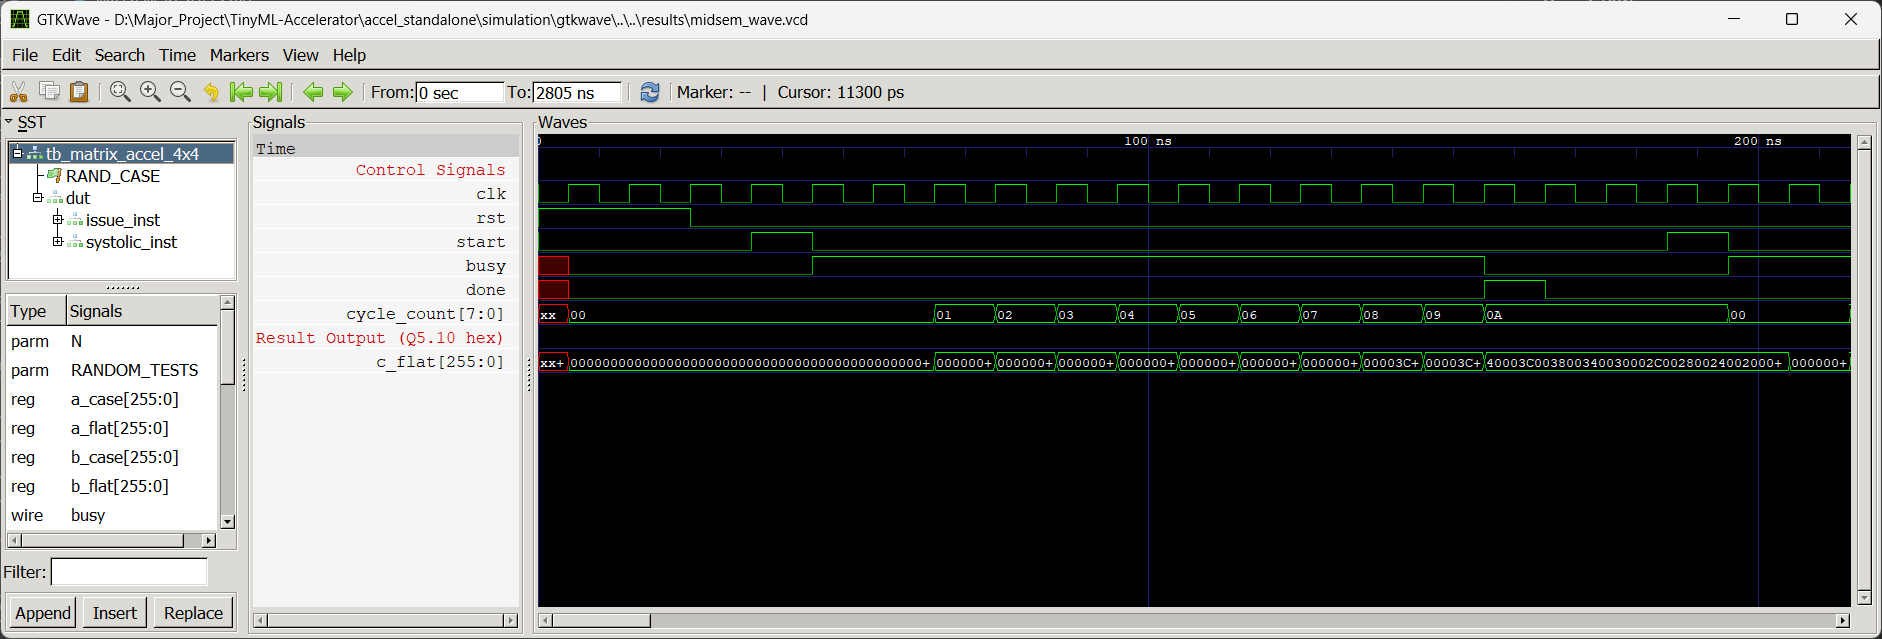
\includegraphics[width=\textwidth]{figures/accelerator_standalone_wave.png}
\caption{GTKWave waveform from the standalone accelerator regression.
         \textit{Control Signals} group (top): \texttt{clk}, \texttt{rst}, \texttt{start}, \texttt{busy}, \texttt{done}.
         \texttt{cycle\_count[7:0]} increments from \texttt{00} to \texttt{0A} (decimal~10),
         confirming the data-independent 10-cycle systolic latency.
         \texttt{c\_flat[255:0]} transitions to the packed Q5.10 result matrix upon \texttt{done} assertion.}
\label{fig:accel_waveform}
\end{figure}
% ----------------------------------------------------------------
\section{Layer 2 --- System-Level Integration Verification}
% ----------------------------------------------------------------

The second layer introduces the full system: PicoRV32 processor, PCPI coprocessor wrapper, and the matrix accelerator.
Firmware compiled for the RISC-V ISA is loaded into simulation memory, and the CPU executes the complete instruction stream that includes the custom accelerator-invoke instruction.

\subsection{Custom Instruction Encoding}

The firmware invokes the matrix multiply accelerator with a single custom instruction:

\begin{lstlisting}[language={}]
# Firmware: invoke the EdgeMATX accelerator
# rs1 = base address of matrix A in memory
# rs2 = base address of matrix B in memory
.word 0x5420818b     # custom-0 opcode: triggers PCPI coprocessor
\end{lstlisting}

The opcode \texttt{0x5420818b} uses the custom-0 opcode space (\texttt{0001011}), which the CPU does not natively decode but instead forwards to the PCPI interface.
The PCPI wrapper captures \texttt{pcpi\_rs1} and \texttt{pcpi\_rs2} as the base addresses of matrices $A$ and $B$, then drives the accelerator datapath.

The corresponding C firmware uses inline assembly to emit the same opcode:

\begin{lstlisting}[language=C]
/* C firmware: invoke accelerator */
asm volatile (
    ".word 0x5420818b\n"
    : /* no outputs */
    : /* no inputs  */
    : "memory"                   /* clobbers memory */
);
\end{lstlisting}

\subsection{PCPI Wrapper Integration Logic}

The wrapper decodes the custom instruction on the PCPI bus and manages the full transaction:

\begin{lstlisting}[language=Verilog]
// PCPI wrapper: detect custom instruction, drive accelerator
always @(posedge clk or posedge rst) begin
    if (rst) begin
        accel_start    <= 0;
        pcpi_wait      <= 0;
        pcpi_ready     <= 0;
    end else begin
        if (pcpi_valid && (pcpi_insn[6:0] == 7'h0b)) begin
            // Custom-0 opcode detected
            matrix_a_base <= pcpi_rs1;  // matrix A base address
            matrix_b_base <= pcpi_rs2;  // matrix B base address
            accel_start   <= 1;
            pcpi_wait     <= 1;         // stall CPU until done
            pcpi_ready    <= 0;
        end
        if (accel_done) begin
            accel_start <= 0;
            pcpi_wait   <= 0;
            pcpi_ready  <= 1;           // release CPU stall
        end
    end
end
\end{lstlisting}

\subsection{Smoke Test (ASM and C Firmware)}

\begin{itemize}
    \item \textbf{Script:} \texttt{run\_pcpi\_demo.ps1}
    \item \textbf{Variants tested:} Assembly firmware and C firmware
    \item \textbf{Result:} PASS (both variants)
    \item \textbf{Date:} 2026-03-05
\end{itemize}

Both variants produced correct output matrix values, validating the complete path: CPU instruction fetch $\rightarrow$ PCPI decode $\rightarrow$ accelerator execution $\rightarrow$ result writeback to memory.

\subsection{Integration Waveform}

Figure~\ref{fig:pcpi_waveform} shows the GTKWave capture from the system-level integration simulation.
The view covers a single accelerator invocation as seen from the CPU-side PCPI bus: the CPU issues custom instruction \texttt{0x5420818b}, which the PCPI wrapper decodes, stalls the processor, runs the accelerator, and releases the stall upon completion.

\begin{figure}[H]
\centering
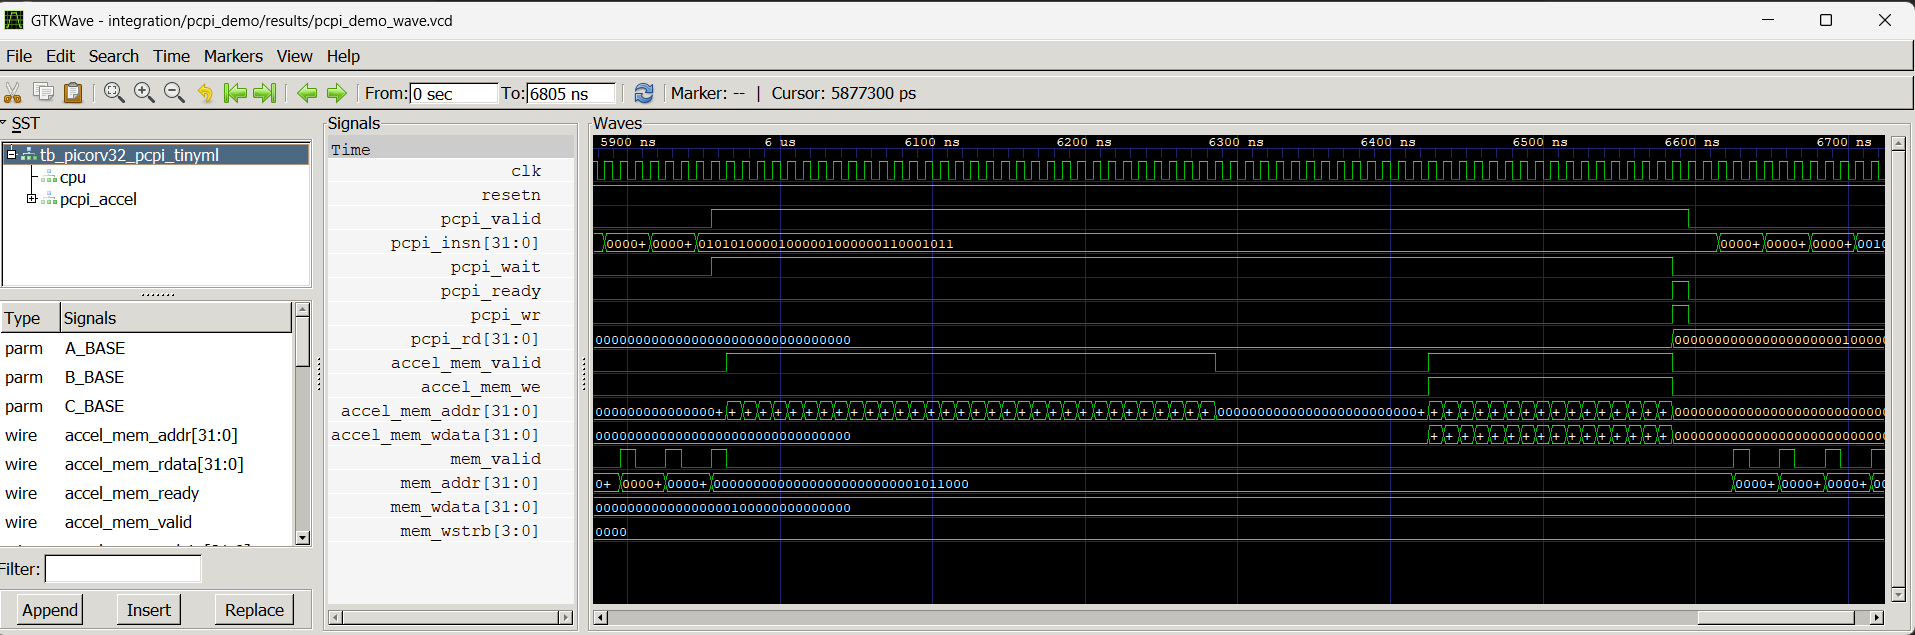
\includegraphics[width=\textwidth]{figures/pcpi_integration_wave.png}
\caption{GTKWave waveform from the PCPI system-level integration simulation.
         \texttt{pcpi\_valid} asserts when the CPU encounters the custom-0 instruction (\texttt{pcpi\_insn = 0x5420818b}).
         \texttt{pcpi\_wait} immediately stalls the processor while the accelerator computes.
         \texttt{accel\_mem\_addr} and \texttt{accel\_mem\_wdata} show the wrapper reading matrix operands from memory.
         \texttt{pcpi\_ready} asserts on completion, releasing the CPU stall and returning control to the instruction stream.}
\label{fig:pcpi_waveform}
\end{figure}

\subsection{8-Case Regression Suite}

\begin{itemize}
    \item \textbf{Script:} \texttt{run\_pcpi\_regression.ps1}
    \item \textbf{Total cases:} 8 distinct matrix input configurations
    \item \textbf{Result:} PASS (8/8)
    \item \textbf{Date:} 2026-03-05
\end{itemize}

The regression suite covers a range of operand types to confirm correctness across the expected input space:

\begin{table}[H]
\centering
\small
\setlength{\tabcolsep}{8pt}
\renewcommand{\arraystretch}{1.3}
\begin{tabular}{lll}
\toprule
\textbf{Case} & \textbf{Description} & \textbf{Result} \\
\midrule
identity\_x\_sequence      & Identity $\times$ sequential integer values & PASS \\
sequence\_x\_sequence      & Sequential $\times$ sequential values       & PASS \\
ones\_x\_sequence          & All-ones matrix $\times$ sequential values  & PASS \\
dense\_random              & Dense non-trivial Q5.10 values              & PASS \\
negative\_elements         & Mixed-sign operand matrices                 & PASS \\
boundary\_values           & Near Q5.10 dynamic range limits             & PASS \\
sparse\_input              & Sparse non-zero entries                     & PASS \\
zero\_matrix               & One operand all-zero                        & PASS \\
\bottomrule
\end{tabular}
\caption{8-case PCPI integration regression results.}
\label{tab:regression_tests}
\end{table}

\subsection{Professor Demonstration Cases}

\begin{itemize}
    \item \textbf{Script:} \texttt{run\_pcpi\_professor\_demo.ps1}
    \item \textbf{Cases:} 5 curated cases
    \item \textbf{Result:} PASS (5/5)
    \item \textbf{Date:} 2026-03-05
\end{itemize}

These cases represent the subset prepared for external review, covering identity multiplication, sequence-based inputs, and dense random inputs with pre-verified expected outputs.

% ----------------------------------------------------------------
\section{Layer 3 --- Protocol Correctness Verification (Handoff Test)}
% ----------------------------------------------------------------

The handoff test validates the PCPI handshake protocol under a mixed instruction stream where \emph{two} consecutive custom-instruction transactions are separated by normal RISC-V instructions.
This test specifically targets protocol robustness: ensuring no stale signals, no state leakage, and correct CPU stall/resume behavior across multiple transactions.

\subsection{PCPI Interface Signals}

\begin{table}[H]
\centering
\small
\setlength{\tabcolsep}{8pt}
\renewcommand{\arraystretch}{1.3}
\begin{tabular}{lll}
\toprule
\textbf{Signal} & \textbf{Direction} & \textbf{Description} \\
\midrule
\texttt{pcpi\_valid} & CPU $\to$ Coprocessor & Custom instruction present on the bus \\
\texttt{pcpi\_insn}  & CPU $\to$ Coprocessor & Full 32-bit instruction word \\
\texttt{pcpi\_rs1}   & CPU $\to$ Coprocessor & Value of source register 1 (matrix A base) \\
\texttt{pcpi\_rs2}   & CPU $\to$ Coprocessor & Value of source register 2 (matrix B base) \\
\texttt{pcpi\_wait}  & Coprocessor $\to$ CPU & Hold CPU stall (computation in progress) \\
\texttt{pcpi\_ready} & Coprocessor $\to$ CPU & Computation complete; resume CPU \\
\texttt{pcpi\_rd}    & Coprocessor $\to$ CPU & Scalar result value (unused in EdgeMATX) \\
\bottomrule
\end{tabular}
\caption{PCPI interface signals.}
\label{tab:pcpi_signals}
\end{table}

\begin{figure}[H]
\centering
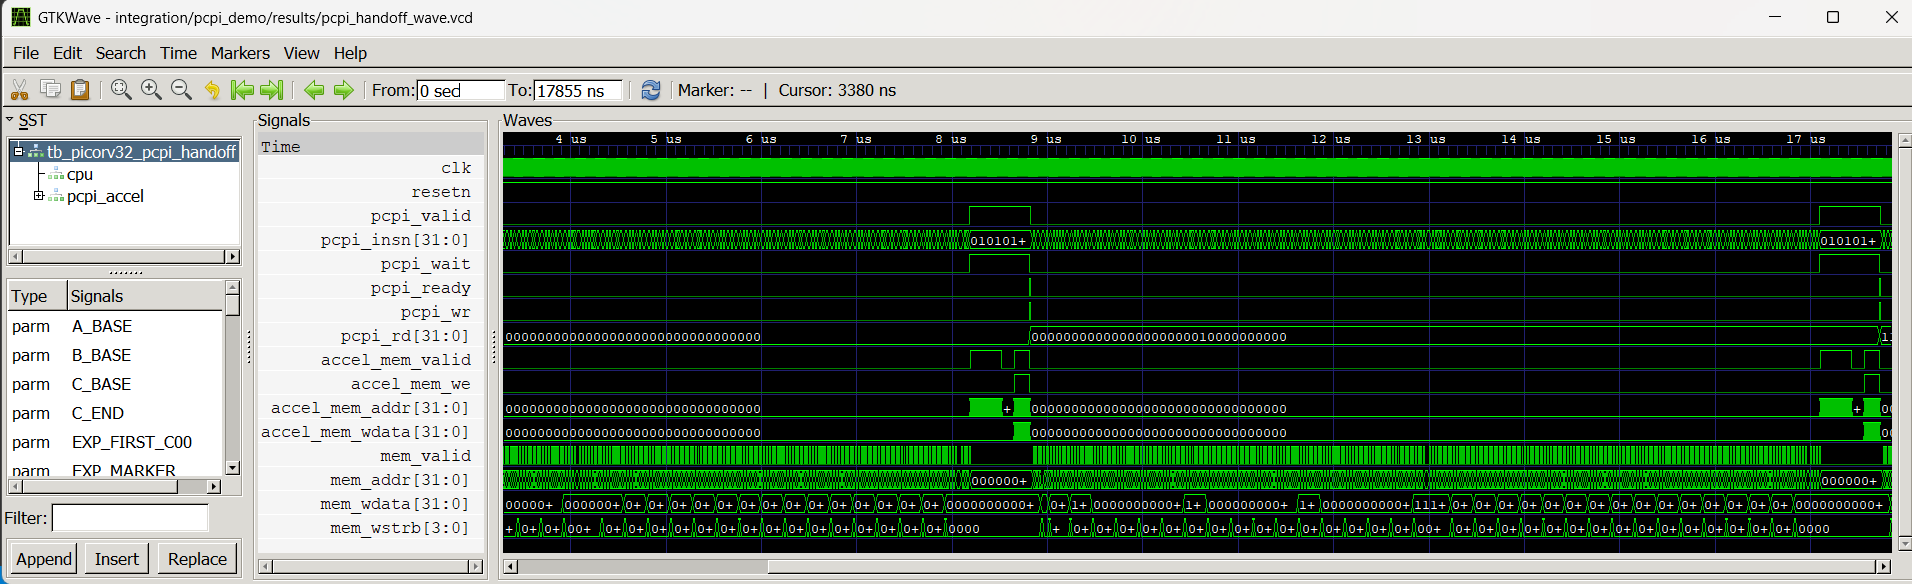
\includegraphics[width=\textwidth]{figures/pcpi_handoff_wave.png}
\caption{GTKWave waveform from the PCPI handoff test, spanning 0--17855\,ns.
         Two distinct custom-instruction transactions are visible (first at $\sim$8\,$\mu$s, second at $\sim$17\,$\mu$s):
         \texttt{pcpi\_valid} asserts when the CPU issues \texttt{0x5420818b};
         \texttt{pcpi\_wait} immediately stalls the CPU while \texttt{accel\_mem\_addr} sequences through the matrix operand addresses;
         \texttt{pcpi\_ready} pulses to release the stall.
         The interval between the two transactions shows normal \texttt{mem\_valid} activity, confirming the CPU resumes instruction execution and no stale signals persist across transactions.}
\label{fig:pcpi_timing}
\end{figure}

\subsection{Handoff Test Results}

\begin{itemize}
    \item \textbf{Script:} \texttt{run\_pcpi\_handoff.ps1}
    \item \textbf{Result:} PASS
    \item \textbf{Date:} 2026-03-05
\end{itemize}

The following protocol counters were observed and validated:

\begin{table}[H]
\centering
\small
\setlength{\tabcolsep}{10pt}
\renewcommand{\arraystretch}{1.3}
\begin{tabular}{lccc}
\toprule
\textbf{Counter} & \textbf{Expected} & \textbf{Observed} & \textbf{Meaning} \\
\midrule
\texttt{custom\_issue\_count}    & 2  & 2  & Custom instructions dispatched by CPU \\
\texttt{ready\_count}           & 2  & 2  & Accelerator completions acknowledged \\
\texttt{wr\_count}              & 2  & 2  & Writeback cycles to result memory \\
\texttt{handshake\_ok\_count}   & 2  & 2  & Full stall+resume cycles validated \\
\texttt{c\_store\_count}        & 32 & 32 & Individual matrix-$C$ element writes ($2 \times 16$) \\
\bottomrule
\end{tabular}
\caption{Handoff test protocol counters: expected vs.\ observed.}
\label{tab:handoff_counters}
\end{table}

These results confirm:

\begin{itemize}
    \item Both custom-instruction transactions were correctly dispatched through PCPI.
    \item The accelerator completed both computations and asserted \texttt{pcpi\_ready} for each.
    \item All 32 output matrix elements ($2 \times 4 \times 4$) were written to memory without corruption.
    \item CPU stalling and resume are clean across multiple instruction boundaries; no state leaks between transactions.
\end{itemize}

% ----------------------------------------------------------------
\section{Layer 4 --- Performance Benchmarking}
% ----------------------------------------------------------------

Performance is measured by comparing the simulation cycle count required to complete a $4 \times 4$ matrix multiplication across three execution configurations:

\begin{enumerate}
    \item \textbf{Hardware-accelerated path:} PCPI active, custom instruction, software multiply disabled in the CPU.
    \item \textbf{Software baseline (no MUL):} PCPI disabled, rv32i ISA, no hardware multiplier.
    \item \textbf{Software baseline (MUL enabled):} PCPI disabled, rv32im ISA, hardware multiply extension active.
\end{enumerate}

The measurement window starts when the firmware issues the computation trigger (custom instruction or software loop entry) and ends when the firmware writes the sentinel value to address \texttt{0x00000000}, which signals end of computation.
This is captured by the testbench as:

\begin{lstlisting}[language={}]
// Testbench cycle measurement output
$display("TB_CYCLES matmul_to_sentinel_cycles=%0d", cycle_counter);
\end{lstlisting}

Automation scripts parse this line, extract the cycle value, and compute speedup ratios.

\subsection{Benchmark Case: \texttt{identity\_x\_sequence}}

\begin{table}[H]
\centering
\small
\setlength{\tabcolsep}{5pt}
\renewcommand{\arraystretch}{1.4}
\begin{tabular}{p{0.34\textwidth}p{0.30\textwidth}p{0.10\textwidth}r}
\toprule
\textbf{Execution Path} & \textbf{Build Configuration} & \textbf{ISA} & \textbf{Cycles} \\
\midrule
Hardware accelerator (EdgeMATX)  & \texttt{ENABLE\_PCPI=1, ENABLE\_MUL=0} & rv32i  &    673 \\
Software baseline (no MUL)  & \texttt{ENABLE\_PCPI=0, ENABLE\_MUL=0} & rv32i  & 26{,}130 \\
Software baseline (MUL)     & \texttt{ENABLE\_PCPI=0, ENABLE\_MUL=1} & rv32im &  7{,}975 \\
\bottomrule
\end{tabular}
\caption{Measured simulation cycle counts for the \texttt{identity\_x\_sequence} benchmark.}
\label{tab:cycle_comparison}
\end{table}

\subsection{Derived Speedups}

\begin{table}[H]
\centering
\small
\setlength{\tabcolsep}{10pt}
\renewcommand{\arraystretch}{1.4}
\begin{tabular}{lcc}
\toprule
\textbf{Comparison} & \textbf{Ratio} & \textbf{Speedup} \\
\midrule
Accelerator vs.\ software no-MUL   & $26{,}130 / 673$ & $\mathbf{38.83\times}$ \\
Accelerator vs.\ software MUL      & $7{,}975  / 673$ & $\mathbf{11.85\times}$ \\
Software MUL vs.\ software no-MUL  & $26{,}130 / 7{,}975$ & $3.28\times$ \\
\bottomrule
\end{tabular}
\caption{Derived speedup values for the \texttt{identity\_x\_sequence} benchmark case.}
\label{tab:speedups_identity}
\end{table}

\begin{figure}[H]
\centering
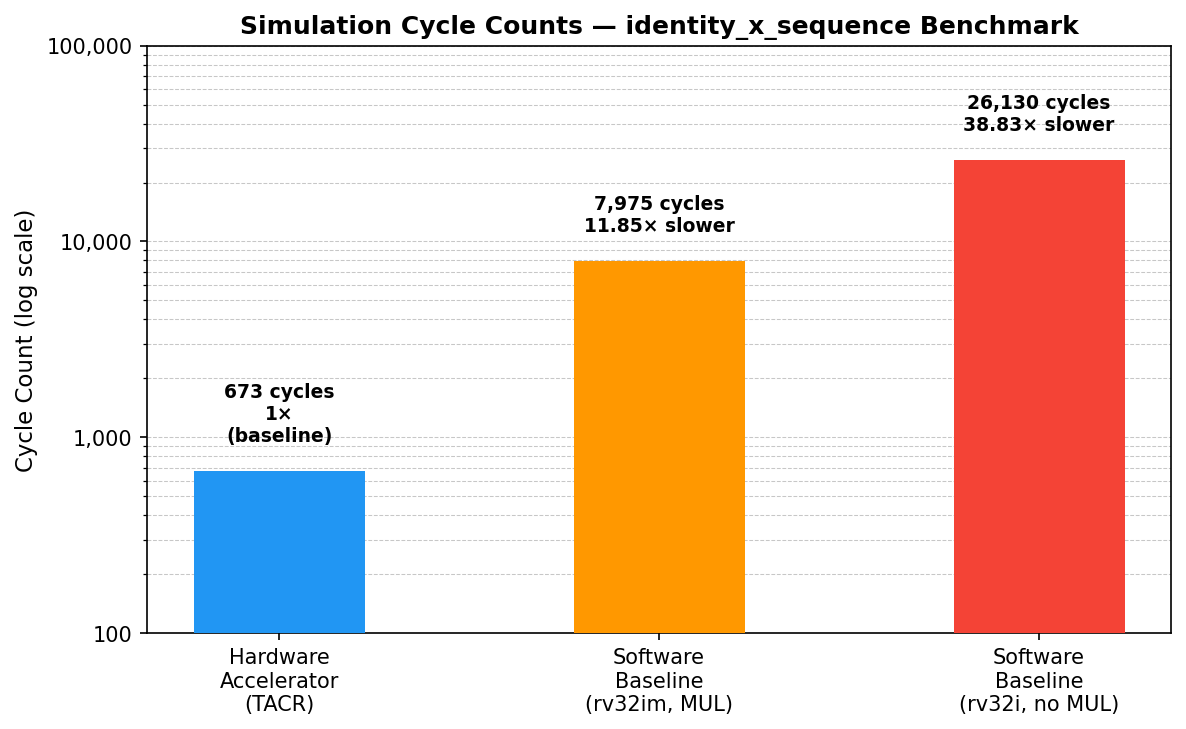
\includegraphics[width=0.88\textwidth]{figures/cycle_count_bar.png}
\caption{Simulation cycle counts across the three execution paths (\texttt{identity\_x\_sequence} case).
         Log-scale Y-axis makes the 673-cycle accelerator bar visible alongside the 26{,}130-cycle software baseline.}
\label{fig:cycle_bar}
\end{figure}

\subsection{Dense Data Profile (\texttt{live\_real\_input.json})}

For the dense checked-in real-input profile, which contains non-trivial Q5.10 values with higher average operand magnitude, the following cycle counts were measured:

\begin{table}[H]
\centering
\small
\setlength{\tabcolsep}{8pt}
\renewcommand{\arraystretch}{1.3}
\begin{tabular}{lrr}
\toprule
\textbf{Execution Path} & \textbf{Cycles} & \textbf{Speedup vs Accelerator} \\
\midrule
Hardware accelerator (EdgeMATX) & 673        & ---            \\
Software baseline (no MUL)  & 36{,}246   & $53.86\times$  \\
Software baseline (MUL)     & 7{,}975    & $11.85\times$  \\
\bottomrule
\end{tabular}
\caption{Cycle counts for the dense \texttt{live\_real\_input.json} profile.}
\label{tab:dense_profile}
\end{table}

The dense profile achieves a \textbf{50x-class speedup} ($53.86\times$) over the rv32i no-MUL baseline because dense operands require a higher instruction count in the shift-and-add software multiply path, while the hardware accelerator's cycle count is \emph{data-independent}---it always completes in 673 cycles regardless of operand values.

\begin{figure}[H]
\centering
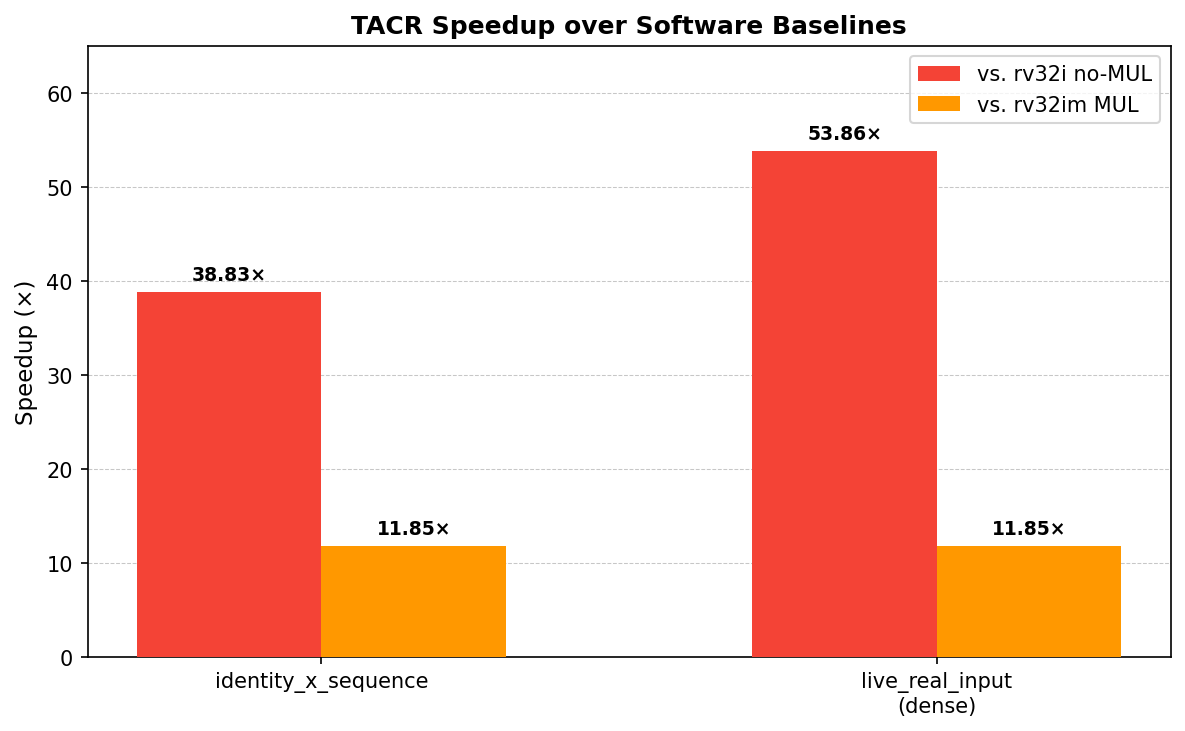
\includegraphics[width=0.88\textwidth]{figures/speedup_comparison.png}
\caption{Speedup achieved by EdgeMATX across the two benchmark profiles.
         The MUL-baseline speedup (11.85$\times$) is data-independent, while the no-MUL speedup increases with operand density (38.83$\times$ to 53.86$\times$) because the shift-and-add software path requires more instructions for larger values.}
\label{fig:speedup_chart}
\end{figure}

\subsection{Why the Acceleration Is Effective}

\paragraph{Against the no-MUL software baseline:}
The rv32i software path has no hardware multiply instruction.
Each of the 16 inner-product accumulations in the $4 \times 4$ multiply requires a multi-instruction shift-and-add sequence.
The hardware accelerator replaces the entire nested loop with a single PCPI transaction, amortizing the fixed interface overhead (memory reads, accelerator start, writeback) across all 16 outputs in one shot.

\paragraph{Against the MUL-enabled software baseline:}
Even with \texttt{ENABLE\_MUL=1} and \texttt{rv32im} firmware, the software path still executes a 3-level nested loop with per-element instruction fetch and dispatch overhead.
The accelerator eliminates this loop overhead entirely.
The $11.85\times$ residual speedup reflects the loop-control and memory-access instruction overhead that remains in the software path even after multiply cost is reduced.

\paragraph{Data-independence of the accelerator:}
The hardware accelerator's cycle count (673) is invariant to the numerical values of the input matrices.
This provides predictable, worst-case-bound execution latency, which is a desirable property for real-time systems.

\subsection{Measurement Fairness}

\begin{itemize}
    \item All three execution paths use \emph{identical input matrix data} for each comparison run.
    \item The MUL baseline requires \emph{both} \texttt{ENABLE\_MUL=1} in the PicoRV32 core \emph{and} firmware compiled as \texttt{rv32im}; enabling only one of the two does not activate the hardware multiply path.
    \item Cycle counts are parsed from the \texttt{TB\_CYCLES} log line and not manually observed.
\end{itemize}

% ----------------------------------------------------------------
\section{Consolidated Verification Summary}
% ----------------------------------------------------------------

\begin{table}[H]
\centering
\small
\setlength{\tabcolsep}{8pt}
\renewcommand{\arraystretch}{1.4}
\begin{tabularx}{\textwidth}{
  >{\raggedright\arraybackslash}X
  >{\ttfamily\raggedright\arraybackslash}X
  >{\centering\arraybackslash}p{2.4cm}
  >{\centering\arraybackslash}p{2.4cm}
}
\toprule
\textbf{Flow} & \textbf{Script} & \textbf{Date} & \textbf{Result} \\
\midrule
Standalone hardening  & run\_midsem\_sim            & 2026-03-05 & PASS (19/19) \\
Smoke ASM/C           & run\_pcpi\_demo             & 2026-03-05 & PASS \\
8-case regression     & run\_pcpi\_regression       & 2026-03-05 & PASS (8/8) \\
Handoff test          & run\_pcpi\_handoff          & 2026-03-05 & PASS \\
Professor cases       & run\_pcpi\_professor\_demo  & 2026-03-05 & PASS (5/5) \\
One-command gate      & run\_pcpi\_local\_check     & 2026-03-05 & PASS \\
\bottomrule
\end{tabularx}
\caption{Consolidated functional validation status across all verification layers.}
\label{tab:consolidated_results}
\end{table}

\begin{table}[H]
\centering
\small
\setlength{\tabcolsep}{8pt}
\renewcommand{\arraystretch}{1.4}
\begin{tabular}{lcc}
\toprule
\textbf{Comparison} & \textbf{Speedup --- identity case} & \textbf{Speedup --- dense case} \\
\midrule
Accelerator vs.\ software (no MUL) & $38.83\times$ & $53.86\times$ \\
Accelerator vs.\ software (MUL)    & $11.85\times$ & $11.85\times$ \\
\bottomrule
\end{tabular}
\caption{Performance summary: speedup across both benchmark profiles.}
\label{tab:speedup_summary}
\end{table}

Key observations:

\begin{itemize}
    \item The hardware accelerator achieves at minimum $11.85\times$ speedup even when compared against a software path equipped with a hardware multiplier.
    \item Against a plain rv32i core, speedup reaches $38$--$54\times$ depending on input data density.
    \item The accelerator cycle count (673 cycles) is invariant to operand values, providing deterministic execution latency.
    \item A single custom instruction replaces the entire $4 \times 4$ nested-loop execution in the CPU, and all result elements are produced and committed to memory within one PCPI transaction.
\end{itemize}

% ----------------------------------------------------------------
\section{Current Limitations and Pending Measurements}
% ----------------------------------------------------------------

The verification evidence at this stage is entirely simulation-based.
The following items remain before the project reaches full hardware closure:

\begin{itemize}
    \item \textbf{FPGA deployment:} The design has not yet been mapped to a physical FPGA target (Pynq-Z2).
          Post-synthesis timing, LUT / DSP48 resource utilization, BRAM usage, and on-board power measurements are not yet available.

    \item \textbf{On-board cycle validation:} Simulation-derived cycle counts will need to be cross-checked against hardware cycle counter measurements (e.g., via PicoRV32 \texttt{rdcycle} CSR) once the design is deployed on the Pynq-Z2.

    \item \textbf{Cycle estimator calibration:} The cycle-scaling estimator tool retains an older accelerator anchor of 869 cycles; the latest measured value is 673 cycles.
          This discrepancy should be corrected before hardware-phase estimation is used.

    \item \textbf{Memory bandwidth characterization:} Current measurements include time for the PCPI wrapper's software-driven memory reads of the input matrices.
          When these are replaced by BRAM-backed access on the FPGA, the memory-access contribution to the cycle count may change.
\end{itemize}

These gaps do not affect the correctness evidence; all functional verification layers pass.
Closing the hardware measurement gap is the single remaining objective of the next project phase.


\chapter{Conclusion}

The EdgeMATX project has reached a complete and reproducible simulation-stage milestone.
The core design---a Q5.10 fixed-point $4 \times 4$ systolic array accelerator tightly coupled to a PicoRV32 core via the PCPI custom-instruction interface---has been fully verified through a four-layer simulation campaign: standalone unit tests (19/19 passing), CPU-integration regression (8/8 cases), protocol handoff validation, and quantified cycle-count benchmarking against two software baselines.

The measured performance results establish the value of the hardware approach: the accelerator delivers a $38.83\times$--$53.86\times$ speedup over a plain rv32i software baseline and $11.85\times$ speedup even against a MUL-equipped rv32im core, with a deterministic 673-cycle execution time independent of input data values.

The single remaining objective is hardware closure: deploying the proven simulation contract onto the Pynq-Z2 FPGA platform, measuring on-board cycle counts, and capturing post-synthesis timing, resource utilization, and power data.
The simulation-based verification framework, firmware, and automation scripts developed in this phase serve as the direct baseline for board-level validation.

\bibliographystyle{IEEEtran}
\bibliography{tacr_references}
\end{document}
